
\documentclass[english]{article}
\usepackage[T1]{fontenc}
\usepackage[utf8]{inputenc}
\usepackage{babel}
\usepackage{geometry}
\usepackage{setspace}

\geometry{verbose,tmargin=3cm,bmargin=3.2cm,lmargin=2.4cm,rmargin=2.4cm}
\linespread{1.0}

\newif\ifjmlrformat
\jmlrformatfalse



% The following packages can be found on http:\\www.ctan.org
%\usepackage{graphics} % for pdf, bitmapped graphics files
%\usepackage{epsfig} % for postscript graphics files
%\usepackage{mathptmx} % assumes new font selection scheme installed
%\usepackage{times} % assumes new font selection scheme installed
\usepackage{amsmath}
\usepackage{amssymb}
\usepackage{amsthm}
\usepackage{mathtools}
\usepackage{bm}
\usepackage{bbm}
\usepackage{euscript}
\usepackage{pifont}
\usepackage{xspace}
\usepackage{xcolor}
\usepackage{graphicx}
\usepackage{tikz}
\usetikzlibrary{arrows.meta,calc}
\usepackage[ruled,vlined]{algorithm2e}
\usepackage{algorithmic}
\renewcommand{\algorithmiccomment}[1]{\hfill$\triangleright$ #1}
\makeatletter
\let\NAT@parse\undefined
\makeatother
\usepackage[numbers,sort&compress]{natbib}
\usepackage[capitalize,noabbrev]{cleveref}

% Adaptive project paths: works when compiling either from the project root or
% from the cdc2026_template directory.
\newcommand{\projectbibfile}{}
\newcommand{\projectstructuralbibfile}{}
\newcommand{\projectfigurepath}{}
\newcommand{\projectappendixpath}{}
\IfFileExists{tools/shared.tex}{%
  \input{tools/shared}%
  \renewcommand{\projectbibfile}{tools/refers}%
  \renewcommand{\projectstructuralbibfile}{tools/dca_structural_complexity_refs}%
  \renewcommand{\projectfigurepath}{figure}%
  \renewcommand{\projectappendixpath}{cdc2026_template/appendices}%
}{%
  \IfFileExists{../tools/shared.tex}{%
    \input{../tools/shared}%
    \renewcommand{\projectbibfile}{../tools/refers}%
    \renewcommand{\projectstructuralbibfile}{../tools/dca_structural_complexity_refs}%
    \renewcommand{\projectfigurepath}{../figure}%
    \renewcommand{\projectappendixpath}{appendices}%
  }{%
    \PackageError{cdc2026-template}{Cannot find tools/shared.tex}{Compile from the project root or from cdc2026_template.}%
  }%
}
\IfFileExists{\projectbibfile.bib}{}{%
  \PackageError{cdc2026-template}{Cannot find \projectbibfile.bib}{Check the adaptive bibliography path.}%
}
\IfFileExists{\projectstructuralbibfile.bib}{}{%
  \PackageError{cdc2026-template}{Cannot find \projectstructuralbibfile.bib}{Check the adaptive structural bibliography path.}%
}
\graphicspath{{figure/}{../figure/}}

\newtheorem{theorem}{Theorem}[section]
\newtheorem{lemma}{Lemma}[section]
\newtheorem{corollary}{Corollary}[section]
\newtheorem{proposition}{Proposition}[section]
\newtheorem{definition}{Definition}[section]
\newtheorem{assumption}{Assumption}[section]
\newtheorem{example}{Example}[section]
\newtheorem{remark}{Remark}[section]
\Crefname{theorem}{Theorem}{Theorems}
\Crefname{lemma}{Lemma}{Lemmas}
\Crefname{corollary}{Corollary}{Corollaries}
\Crefname{proposition}{Proposition}{Propositions}
\Crefname{definition}{Definition}{Definitions}
\Crefname{assumption}{Assumption}{Assumptions}
\Crefname{example}{Example}{Examples}
\Crefname{remark}{Remark}{Remarks}

\title{\LARGE \bf
Revising DC 
}

%\author{ \parbox{3 in}{\centering Huibert Kwakernaak*
%         \thanks{*Use the $\backslash$thanks command to put information here}\\
%         Faculty of Electrical Engineering, Mathematics and Computer Science\\
%         University of Twente\\
%         7500 AE Enschede, The Netherlands\\
%         {\tt\small h.kwakernaak@autsubmit.com}}
%         \hspace*{ 0.5 in}
%         \parbox{3 in}{ \centering Pradeep Misra**
%         \thanks{**The footnote marks may be inserted manually}\\
%        Department of Electrical Engineering \\
%         Wright State University\\
%         Dayton, OH 45435, USA\\
%         {\tt\small pmisra@cs.wright.edu}}
%}

\ifjmlrformat
\author{\name Luxuan Li \email luxuanli@buaa.edu.cn \\
       \addr School of Mathematical Sciences\\
       Beihang University\\
       Beijing 100191, China
       \AND
       \name Chunfeng Cui \email chunfengcui@buaa.edu.cn \\
       \addr School of Mathematical Sciences\\
       Beihang University\\
       Beijing 100191, China
       \AND
       \name Xiao Wang \email wangx936@mail.sysu.edu.cn \\
       \addr School of Computer Science and Engineering\\
       Sun Yat-sen University\\
       Guangzhou 510006, China}
\else
\author{
       Luxuan Li\\
       School of Mathematical Sciences\\
       Beihang University\\
       Beijing 100191, China\\
       \texttt{luxuanli@buaa.edu.cn}
       \and
       Chunfeng Cui\\
       School of Mathematical Sciences\\
       Beihang University\\
       Beijing 100191, China\\
       \texttt{chunfengcui@buaa.edu.cn}
       \and
       Xiao Wang\\
       School of Computer Science and Engineering\\
       Sun Yat-sen University\\
       Guangzhou 510006, China\\
       \texttt{wangx936@mail.sysu.edu.cn}
       }
\fi


\begin{document}



\maketitle


%%%%%%%%%%%%%%%%%%%%%%%%%%%%%%%%%%%%%%%%%%%%%%%%%%%%%%%%%%%%%%%%%%%%%%%%%%%%%%%%
\begin{abstract}
In this paper, we study a general class of nonconvex DC constrained problems , where the feasible set is possibly nonconvex, and the concave part of the DC objective is allowed to be nonsmooth. The fundamental challenge lies in maintaining feasibility for nonconvex constraints while achieving favorable oracle complexity.

\ifjmlrformat
\begin{keywords}
Nonsmooth optimization, DC optimization, constrained optimization, penalty methods, smoothing approximation, momentum, oracle complexity
\end{keywords}
\else
\noindent\textbf{Keywords:} Nonsmooth nonconvex optimization,  constrained optimization, DC optimization, penalty methods, smoothing approximation, momentum, oracle complexity.
\fi


\end{abstract}


%%%%%%%%%%%%%%%%%%%%%%%%%%%%%%%%%%%%%%%%%%%%%%%%%%%%%%%%%%%%%%%%%%%%%%%%%%%%%%%%

\section{INTRODUCTION}
In this paper, we study a class of nonsmooth nonconvex constrained
optimization problems formulated as
\begin{equation}
\tag{{\bf P}}
\label{prob:main}
\begin{alignedat}{3}
   \min\limits_{\bx \in \RR^n} \quad
      & F(\bx) &&:= \Phi(\bx) - g(\bx),\\
   \text{s.t.} \quad
      & \bc_{\calE}(\bx) &&= \zero, \\
      & \bc_{\calI}(\bx) &&\leq \zero ,
\end{alignedat}
\end{equation}
where the objective $F = \Phi - g$ has a \emph{difference-of-convex}
(DC) structure: $\Phi:\RR^n\to\RR\cup\{+\infty\}$ and
$g:\RR^n\to\RR\cup\{+\infty\}$ are proper closed convex functions, and
$g$ is allowed to be nonsmooth, so that $F$ is in general both
nonsmooth and nonconvex. The constraint mappings
$\bc_{\calE}:\RR^n\to\RR^{m_{\calE}}$ and
$\bc_{\calI}:\RR^n\to\RR^{m_{\calI}}$ are continuously differentiable
and define a nonempty feasible set
$\calX = \{\bx \in \RR^n : \bc_{\calE}(\bx) = \zero,\
\bc_{\calI}(\bx) \le \zero\}$.

Two settings motivate our study of Problem~\eqref{prob:main}. The first is deterministic constrained DC programming, in which both
$\Phi$ and $g$ can be evaluated exactly. DC functions form a vector
space and constitute a remarkably rich subclass of locally Lipschitz
nonconvex functions \citep{Zhang-2020-Complexity,kong2024cost,davis2022gradient}; the formulation subsumes smooth nonconvex minimization ($g \equiv 0$) as a
trivial instance and covers a broad spectrum of classical
applications, including nonconvex quadratic programming
\citep{lethi1997solving,lethi1998branch}, convex--concave programming
\citep{yuille2003concave,shen2016disciplined}, kernel selection \citep{argyriou2006dc},
and bilevel programming \citep{lethi2009dc}. While the unconstrained DC
objective is by now well understood, the nonlinear constraints
$\bc_{\calE}$ and $\bc_{\calI}$, which arise naturally from
structural or resource requirements such as energy budgets in deep
network compression \citep{yang2019ecc,chen2018constraint} and safety
constraints in control \citep{paternain2019constrained},introduce
severe geometric complications of their own.

A second motivation for \eqref{prob:main} is regularized empirical risk minimization in large-scale machine learning. The DC structure of the objective naturally captures the combination of a data-fitting risk and a nonconvex regularizer. Specifically, any smooth nonconvex loss can be reformulated as a DC function by adding and subtracting a strongly convex quadratic term. Moreover, popular nonconvex regularizers such as the capped-$\ell_1$ penalty \citep{zhang2010analysis} and SCAD \citep{fan2001variable} admit explicit DC decompositions $r = r_{\mathrm{cvx}} - g$. In large-scale training, the data-fitting component in $\Phi$ is a
population risk accessible only through stochastic gradients under
data sampling, whereas the subtracted component $g$, which collects
the concave part of the regularizer, remains a fixed deterministic
function. 

To ground our framework, we provide two concrete motivating examples that can be formulated as instances of Problem~\eqref{prob:main}:

\subsection{Motivating Examples}

\begin{enumerate}
  \item \textbf{Deterministic DC objective (min-structured loss).}
Losses given by a pointwise minimum of convex functions are
intrinsically DC, via the identity
$\min\limits_{k\le K} a_k=\sum_{k=1}^{K}a_k-\max\limits_{k\le K}\sum_{j\ne k}a_j$
for convex $a_1,\dots,a_K$. For instance, in piecewise-affine
(clusterwise) regression, each observation is explained by the best of
$K$ candidate affine models,
\[
   \min\limits_{\bw_1,\dots,\bw_K}\ \sum_{i=1}^{N}\,
   \min\limits_{1\le k\le K}\bigl|y_i-\langle \bw_k,\bx_i\rangle\bigr|,
\]
and applying the identity samplewise yields $F=\Phi-g$ with
$\Phi(\bw)=\sum_{i,k}|y_i-\langle \bw_k,\bx_i\rangle|$ and
$g(\bw)=\sum_{i}\max\limits_{k}\sum_{j\ne k}|y_i-\langle \bw_j,\bx_i\rangle|$.
Both components are convex, piecewise affine, and nonsmooth, with
subgradients available in closed form.

  \item \textbf{Stochastic nonconvex regularized ERM.}
  Consider a convex data-fitting loss $\ell$ coupled with a capped-$\ell_1$ penalty:
  \[
     \min\limits_{\bx}\ \underbrace{\EE_{\xi}[\ell(\bx,\xi)] + \lambda\|\bx\|_1}_{\Phi(\bx)}
     \;-\;\underbrace{\lambda\sum_i\max\limits\{|x_i|-\theta,0\}}_{g(\bx)}.
  \]
  Here, the data-fitting component $\Phi$ is a population risk evaluated solely via stochastic gradients, whereas the subtracted penalty $g$ is a fixed, deterministic, and nonsmooth convex function whose subgradients can be computed in closed form.
\end{enumerate}

\subsection{Related Work}
\label{subsec:known-and-open}

\paragraph{Non-asymptotic rates for DC optimization.}

Removing differentiability of the subtracted component $g$ has been a
central theme in DC programming. Recent non-asymptotic analyses have
made this theme quantitative, but their guarantees are expressed through
different decomposition-dependent certificates. For DCA and CCCP-type
methods, rates are usually stated in terms of objective decrease, step
lengths, or critical-distance proxies under additional smoothness or
curvature assumptions
\citep{yurtsever2022cccp,abbaszadehpeivasti2023rate}. Projection-free
DC methods over compact convex domains instead use Frank--Wolfe-type
linear minimization gaps \citep{khamaru2018convergence,maskan2025}.
Stochastic DC methods use critical-distance criteria or one-sided gap
functions, often with a smooth or variance-reduced stochastic component
\citep{xu2019stochastic,le2022stochastic,nguyen2025improved}. These
certificates are value-typed or algorithm-dependent, while the exact DC
residual
\[
    \operatorname{dist}\bigl(\zero,\partial\Phi(\bx)-\partial g(\bx)\bigr)
\]
is norm-typed and same-point. Passing from a gap bound to a residual
bound therefore changes units, typically through a square-root relation.
Existing finite-time results hence do not settle whether exact
same-point $\epsilon$-criticality is itself attainable for nonsmooth DC
pairs. The first question is therefore:

\emph{Is $\epsilon$-criticality finite-time attainable in DC
optimization? If not, does a unified single notion exist that relaxes it while
remaining both finite-time attainable and sound?}

\paragraph{Non-asymptotic rates for unconstrained nonsmooth nonconvex
optimization.}
For general Lipschitz objectives, $\epsilon$-Clarke stationarity is
unattainable in finite time \citep{Zhang-2020-Complexity}, while the
structure-blind Goldstein $(\delta,\epsilon)$-stationarity relaxation admits
$O(\delta^{-1}\epsilon^{-3})$ guarantees
\citep{Zhang-2020-Complexity,davis2022gradient},
one $\epsilon$-factor away from the $O(\epsilon^{-2})$ smooth
benchmark. These results treat the objective as a black box. 

The second question is therefore:

\emph{Under an finite-sum attainable targat of DC
criticality, can the DC structure be provably exploited to match the
$O(\epsilon^{-2})$ rate of unconstrained smooth nonconvex
optimization?}

\paragraph{Constrained nonconvex optimization.}
The rates above are established either without constraints or over
simple convex compact sets accessed through projections or linear
minimization oracles \citep{khamaru2018convergence,maskan2025}; general nonlinear
constraints are handled by penalty or augmented-Lagrangian schemes
whose inner solves make the methods double-loop and couple the inner
accuracy to the outer complexity
\citep{xie2021complexity,lu2022penalty,yu2021convergence,kanzow2025adaptive}. The third question is:

\emph{can a single-loop method, free of inner solvers and
backtracking, retain the optimal $O(\epsilon^{-3})$ complexity under general
nonlinear, possibly nonconvex, constraints? (ALM)}

\subsection{Contributions}
We tackle the three question for Problem~\eqref{prob:main} when both components of the DC decomposition may be nonsmooth.  This class is rich enough to cover
constrained DC programs and nonconvex-regularized empirical risk
minimization. At first sight, the DC structure makes the search for
stationary points easier on both sides of the oracle--target ledger:
the natural target, DC criticality
$\zero\in\partial\Phi(\bx)-\partial g(\bx)$, is strictly weaker than
Clarke stationarity, and the natural oracle, returning values and
subgradients of $\Phi$ and $g$ separately, is strictly stronger than
a Clarke subgradient oracle. Surprisingly, even with a weaker target
and a stronger oracle, finding an $\epsilon$-critical point, i.e., a
point $\bar\bx$ with
$\operatorname{dist}(\zero,\partial\Phi(\bar\bx)-\partial g(\bar\bx))
\le\epsilon$, is intractable. In other words, no algorithm
interacting with the component-wise DC oracle can guarantee an
$\epsilon$-critical point among its queried iterates within a finite
number of oracle calls.This intractability suggests that, to obtain meaningful
non-asymptotic results for DC problems, we need to refine the notion
of criticality. We then introduce such a unified notion and base our analysis on
it, leading to the following main contributions:

\begin{itemize}
\item We show that a traditional $\epsilon$-critical point cannot be
obtained in finite time, even under the strong component-wise DC
oracle, returning values and subgradients of $\Phi$ and $g$
separately.


\item We study $(\delta_\Phi,\delta_g,\epsilon)$-critical points
(\Cref{def:delta-eps-critical}), which unify existing relaxations of
DC criticality.For smooth DC functions, this notion reduces to the usual
$\epsilon$-stationarity by  choosing \(\delta_\Phi=O(\epsilon^2/L_\Phi)\) and \(\delta_g=O(\epsilon^2/L_g)\).

\item For unconstrained DC optimization, we show that proximal DCA returns a \((0,\delta_g,\epsilon)\)-critical point within
\(\mathcal O(\max\limits\{\epsilon^{-2},\delta_g^{-2}\})\) subproblem solves,
where the dependence on \(\delta_g\) improves to
\(\mathcal O(\max\limits\{\epsilon^{-2},\delta_g^{-1}\})\) when \(g\) is
\(L_g\)-smooth. \blue{Moreover, if each subproblem is solved inexactly to
accuracy
\[
\omega=
\mathcal O\!\left(
\min\limits\left\{
\eta\epsilon^2,\,
\frac{\delta_\Phi^2}{\eta G_\Phi^2},\,
\frac{\delta_g^2}{\eta G_g^2}
\right\}
\right),
\]
then inexact proximal DCA returns a
\((\delta_\Phi,\delta_g,\mathcal O(\epsilon))\)-critical point with total
inner-iteration complexity
\[
\mathcal O\!\left(
\max\limits\left\{
\frac{\Delta}{\eta\epsilon^2},\,
\frac{\eta\Delta G_g^2}{\delta_g^2}
\right\}
\cdot T_{\rm sub}(\omega)
\right),
\]
where \(T_{\rm sub}(\omega)\) denotes the number of inner iterations
needed to solve one proximal DCA subproblem to accuracy \(\omega\).}

\item We extend the criticality notion to the constrained problem
\eqref{prob:main} and propose a single-loop method attaining a
$(\delta_\Phi,\delta_g,\epsilon)$-critical point in $O(\epsilon^{-2})$
iterations under general nonlinear, possibly nonconvex, constraints
(see \Cref{sec:complexity-analysis}), matching the unconstrained rate above
despite nonsmoothness in both components.
\end{itemize}


\subsection{Notations}
Throughout, $\|\cdot\|$ denotes the Euclidean norm and
$\langle\cdot,\cdot\rangle$ the standard inner product on $\RR^n$. For
a proper closed convex function $h$, $\partial h(\bx)$ denotes its
convex subdifferential, $\partial_\delta h(\bx)$ its
$\delta$-subdifferential, and $h^*$ its Fenchel conjugate; for a
locally Lipschitz $F$, $\partial_C F(\bx)$ denotes the Clarke
subdifferential. We write
$\operatorname{dist}(A,B) := \inf\limits_{\ba\in A,\,\bb\in B}\|\ba-\bb\|$
for nonempty sets $A,B\subseteq\RR^n$, and $\operatorname{dist}(\bv,A)
:= \operatorname{dist}(\{\bv\},A)$. Bold lowercase letters denote
vectors and $\zero$ the zero vector.

\section{Preliminaries}
We introduce the definitions of the Clarke subdifferential and various approximate Clarke stationarity points for general locally Lipschitz functions.

Let $F:\RR^d\to\RR$ be locally Lipschitz. The Clarke subdifferential of
$F$ at $\bx$ is denoted by $\partial_C F(\bx)$~\citep{clarke1990optimization}.
A point $\bx$ is called an $\varepsilon$-Clarke stationary point if
\[
    \operatorname{dist}\bigl(\zero,\partial_C F(\bx)\bigr)
    \leq \varepsilon .
\]
For general nonsmooth nonconvex functions, such a same-point certificate
is not a finite-time target in the worst case. This motivates the
Goldstein-type relaxation below~\citep{goldstein1977optimization,Zhang-2020-Complexity}.

\begin{figure}[t]
    \centering
    \includegraphics[width=\textwidth]{goldstein_vs_approximate_subdifferential.pdf}
   \caption{The Goldstein subdifferential $\partial^G_\delta$ and the
$\delta$-subdifferential $\partial_\delta$ relax exact stationarity along different axes. The former convexifies exact subgradients collected over the ball $\mathcal{B}_\delta(\bar{\bx})$ (a spatial enlargement), while the
latter fixes the base point and tolerates a Fenchel--Young gap of at most
$\delta$ in the supporting inequality (a value relaxation).}
    \label{fig:goldstein-vs-approximate-subdifferential}
\end{figure}

For two sets \(A,B\subseteq\RR^n\), we use the Minkowski difference
\(A-B\), also called the pairwise difference set, defined by
\[
    A-B:=\{\ba-\bb:\ba\in A,\ \bb\in B\}.
\]

\section{Convergence Criteria for Nonsmooth DC Optimization}
\label{sec:dc-convergence-criteria}

We consider the unconstrained difference-of-convex (DC) problem
\begin{equation}
    \min\limits_{\bx\in\RR^n}
    F(\bx):=\phi(\bx)-g(\bx),
    \label{Eq: unconstrained DC problem}
\end{equation}
where $\phi,g:\RR^n\to\RR\cup\{+\infty\}$ are proper, closed, and convex. Both components are allowed to be nonsmooth; notably, we do not assume the differentiability of the concave component $-g$.

\subsection{Criticality and $\varepsilon$-criticality}
\label{sec:finite-time-barrier}
A point $\bar\bx$ is called a \emph{critical point} of Problem~\eqref{Eq: unconstrained DC problem} if
\begin{equation}
    \label{def:dc-critical}
    \zero\in \partial\phi(\bar\bx)-\partial g(\bar\bx).
\end{equation}
Equivalently, there exist $\bu\in\partial\phi(\bar\bx)$ and $\bv\in\partial g(\bar\bx)$ such that $\bu=\bv$. When both convex components are finite and locally Lipschitz around $\bar\bx$, the Clarke calculus gives $\partial_C F(\bar\bx) \subseteq \partial\phi(\bar\bx)-\partial g(\bar\bx)$. Hence, any local minimizer $\bar\bx$ of $F=\phi-g$ satisfies
\[
    \zero\in\partial_C F(\bar\bx) \subseteq \partial\phi(\bar\bx)-\partial g(\bar\bx).
\]

Exact same-point DC criticality is decomposition-dependent and may be
 weaker than Clarke stationarity of the difference function. For
example, let
\[
    \phi(x)=|x|,\qquad g(x)=|x|+x .
\]
Then \(\Psi=\phi-g=-x\), and hence
\[
    \partial_C\Psi(0)=\{-1\},
\]
so \(0\notin\partial_C\Psi(0)\). However,
\[
    \partial\phi(0)=[-1,1],\qquad \partial g(0)=[0,2],
\]
and therefore
\[
    0\in \partial\phi(0)-\partial g(0).
\]
Thus \(x=0\) is DC-critical for this particular decomposition even though
it is not Clarke-stationary for \(\Psi\). This example shows that a
finite-time lower bound for exact DC criticality cannot be obtained by
directly invoking lower bounds for pointwise Clarke stationarity of
\(\Psi\). The lower-bound construction must instead be carried out at the
level of the DC pair \((\phi,g)\) and the residual
\[
    \operatorname{dist}\bigl(0,\partial\phi(x)-\partial g(x)\bigr).
\]
% For this reason, our hard instance is built in two layers. A disjoint-kink
% background pair keeps every queried point's DC residual bounded away from
% zero, by the same resisting-oracle mechanism used at the Clarke level. A
% second, common-kink layer is then grafted onto both convex components at a
% single hidden location: it leaves the objective $F=\phi-g$, its Lipschitz
% constant, and its optimality gap completely unchanged, yet it enlarges
% $\partial\phi(x)-\partial g(x)$ at that location into a set containing
% zero, producing a point that is DC-critical without being Clarke
% stationary for $F$. This second layer is what makes the lower bound
% genuinely exercise the fact that DC criticality is weaker than Clarke
% stationarity, rather than inheriting hardness only because the two notions
% happen to coincide on the instance.

Given $\varepsilon>0$, a natural finite-time goal is the $\varepsilon$-criticality condition:
\begin{equation}
    \label{eq:exact-dc-eps-criticality}
    \operatorname{dist}\!\left( \zero, \partial\phi(\bar\bx)-\partial g(\bar\bx) \right) \le \varepsilon.
\end{equation}
This equivalently requires the existence of $\bu\in\partial\phi(\bar\bx)$ and $\bv\in\partial g(\bar\bx)$ such that $\|\bu-\bv\|\le \varepsilon$.

For comparison, the $\varepsilon$-stationarity condition for a locally Lipschitz nonsmooth nonconvex objective $F$ is $\operatorname{dist}\bigl(\zero,\partial_C F(\bar\bx)\bigr) \le \varepsilon$. Since $\partial_C F(\bar\bx) \subseteq \partial\phi(\bar\bx)-\partial g(\bar\bx)$, we have
\[
    \operatorname{dist}\!\left( \zero, \partial\phi(\bar\bx)-\partial g(\bar\bx) \right) \le \operatorname{dist}\bigl(\zero,\partial_C F(\bar\bx)\bigr).
\]
Thus, \eqref{eq:exact-dc-eps-criticality} serves as a decomposition-dependent DC analogue of Clarke $\varepsilon$-stationarity, and it ism weaker.

Zhang et al.~\citep{Zhang-2020-Complexity} established that for a broad class of Lipschitz nonsmooth nonconvex functions, no finite-time first-order algorithm can guarantee finding a point satisfying $\operatorname{dist}\bigl(\zero,\partial_C F(\bx)\bigr) \le \varepsilon$. For DC optimization, this limitation need to be re-evaluated for two reasons:
\begin{itemize}
\item[(Q1)] \emph{The DC oracle is stronger.} A DCA-type method may
query $\partial\phi$ and $\partial g$ \emph{separately}, and may even
observe $\phi(x)$ and $g(x)$ individually, whereas the obstruction of
\citet[Theorem~5]{Zhang-2020-Complexity} grants only one generalized
gradient of the whole objective. Since more information can only make
the problem easier, the lower bound is not inherited automatically.
\item[(Q2)] \emph{The DC measure is weaker.} The DC calculus gives
$\partial_C(\phi-g)(x)\subseteq\partial\phi(x)-\partial g(x)$, hence
\[
 \operatorname{dist}\bigl(0,\partial\phi(x)-\partial g(x)\bigr)
 \le
 \operatorname{dist}\bigl(0,\partial_C(\phi-g)(x)\bigr).
\]
Thus DC criticality is \emph{easier} to satisfy than Clarke
stationarity, so proving that even this weaker target is unattainable is
a strictly stronger statement than
\citet[Theorem~5]{Zhang-2020-Complexity}, not a corollary of it. A
construction whose DC residual and Clarke residual coincide everywhere
-- such as one built purely from disjoint component kinks -- proves the
Clarke-level statement but never actually tests (Q2), since the DC
target set is never larger than the Clarke target set on such an
instance. The construction below is designed so that (Q2) is tested
directly, at an explicit point where the two residuals differ.
\end{itemize}

The relevant question is whether finite-time $\varepsilon$-criticality can be achieved under this stronger DC oracle. Unfornunately, the answer is negative, as we show next. 
We settle both on a single explicit instance which is different from the hard instance constructed in \cite{Zhang-2020-Complexity}.

We formulate the lower bound under the setting where the pair $(\phi,g)$ is explicitly provided as problem data, granting the algorithm separate access to both convex components. \blue{Throughout this paper, we focus on the following subset of Lipschitz functions. For $\Delta,L,G>0$ and a fixed initial point $\bx^0$, we define:}
\[
\begin{aligned}
\mathcal D(\Delta,L,G) := \Bigl\{ (\phi,g):\;& \phi,g \text{ are proper, closed, convex, and finite-valued},\\
& F:=\phi-g \text{ is } L\text{-Lipschitz and Hadamard directionally differentiable},\\
& F(\bx^0)-\inf\limits_{\bx}F(\bx)\le \Delta,\\
& \sup\limits_{\bx} \sup\limits_{\bu\in\partial\phi(\bx),\,\bv\in\partial g(\bx)} \max\limits\{\|\bu\|,\|\bv\|\} \le G \Bigr\}.
\end{aligned}
\]
We then consider the \emph{strong} DC first-order oracle, which returns
both component values in addition to both component subgradients:
\[
    \mathcal O_{\rm DC}(\bx) = \bigl( \phi(\bx),\,g(\bx),\,\bu,\,\bv \bigr), \qquad \bu\in\partial\phi(\bx),\quad \bv\in\partial g(\bx).
\]
This dominates the weaker oracle $\bigl(F(\bx),\bu,\bv\bigr)$ used above, since $F(\bx)=\phi(\bx)-g(\bx)$ is recoverable from it; a lower bound against $\mathcal O_{\rm DC}$ is therefore the stronger statement required by (Q1). We make this claim precise as follows.
\begin{theorem}
\label{thm:dc-oracle-limitation-sketch}
Fix $\Delta,L,G>0$. There exists an absolute constant $c>0$ such that for every query budget $K\le cG/L$, every $\varepsilon\in(0,L)$, and every algorithm $\mathcal{A}$ interacting with the oracle $\mathcal O_{\rm DC}$, there exists a pair $(\phi,g)\in\mathcal D(\Delta,L,G)$ such that, with probability at least $1/2$, none of the first $K$ points $\{\bx^k\}_{k=1}^K$ queried by $\mathcal{A}$ is $\varepsilon$-critical:
\[
    \operatorname{dist}\!\left(
        \zero,\,
        \partial\phi(\bx^k)-\partial g(\bx^k)
    \right)
    >
    \varepsilon,
    \qquad k=1,\ldots,K.
\]
Moreover, the constructed pair contains a point $s$ with
\[
    \zero\in\partial\phi(s)-\partial g(s),
    \qquad
    \zero\notin\partial_C(\phi-g)(s).
\]
\end{theorem}

\begin{remark}
\label{rmk:GK-tradeoff}
Equivalently, for every $K$ the same construction gives a hard pair in $\mathcal D(\Delta,L,G_K)$ with $G_K=O(KL)$: each hidden background kink forces a slope jump in whichever convex component carries it, and monotonicity of a one-dimensional convex subgradient means these jumps accumulate rather than cancel. This $K$-dependence is specific to the one-dimensional construction; it is not present in the underlying Clarke-level obstruction of \citet{Zhang-2020-Complexity}, which does not need to keep two components separately bounded. 
% Removing the horizon restriction while keeping $G$ fixed for arbitrary $K$ would require a higher-dimensional zero-chain construction, which we leave for future work since the present statement already suffices to motivate the relaxed criticality measure introduced next.
\end{remark}
The hard instance has two layers, detailed in
\Cref{Appendix: Finite-Time Barriers of DC}.
\begin{proof}[Proof sketch]
We first construct a DC pair $(\phi_0,g_0)$ by decompositing the 
resisting-oracle construction in \citet{Zhang-2020-Complexity}.
% : given the
% $K$ queried points, it places hidden kinks between them so that every
% queried point has DC residual equal to a fixed gap $L>\varepsilon$. This
% layer is fixed once its geometric parameter is chosen; no part of it is
% hidden from the algorithm.

A common-kink layer $c_s(x)=M|x-s|+\beta-Ms$ is then added identically to
both components, $\phi_s=\phi_0+c_s$ and $g_s=g_0+c_s$. Because the same
term is added to both sides, $F=\phi_s-g_s=\phi_0-g_0$ is completely
unaffected by $s$: its Lipschitz constant, its optimality gap, and its
Clarke subdifferential everywhere are independent of $s$. Choosing the
intercept $\beta-Ms$ so that $c_s$ agrees with a fixed, $s$-independent
affine function at every point to the left of $s$ makes the entire
strong-oracle transcript -- both component values and both component
subgradients -- identical at every queried point, for every admissible
hidden location $s$ beyond the largest queried point. At $x=s$ itself,
the common kink enlarges $\partial\phi_s(s)-\partial g_s(s)$ into an
interval containing zero while leaving $\partial_C(\phi_s-g_s)(s)$
unchanged, producing the point promised in the theorem.

A two-instance argument over locations $s\neq s'$, both consistent with
the same $K$-query transcript, then shows that no algorithm can
guarantee success against both simultaneously, giving the stated
probability bound.
\end{proof}

\subsection{A Unified Notion of Approximate Criticality}
\label{sec:criticality}
In this section, we propose a unified notion to measure approximate criticality. We first recall the standard \(\delta\)-subdifferential of a proper closed convex function.

If $h:\RR^n\to\RR\cup\{+\infty\}$ is a convex function and $\delta > 0$, then for $\bar{\bx}\in\operatorname{dom} h$, the $\delta$-subdifferential of $h$ at $\bar{\bx}$ is defined by
\[
    \partial_\delta h(\bar{\bx})
    :=
    \left\{
    \bv\in\RR^n:
    h(\bz)\ge h(\bar{\bx})
    +\langle \bv,\bz-\bar{\bx}\rangle-\delta,
    \quad \forall \bz\in\RR^n
    \right\}.
\] 
When $\delta=0$, it reduces to the standard convex subdifferential. 
Figure~\ref{fig:epsilon_subgradient} illustrates that $\delta$ acts as a vertical relaxation of the supporting affine function in the geometric interpretation of the $\delta$-subgradient.

We first record the Fenchel-gap characterization of the
$\delta$-subdifferential below.
\begin{lemma}
\label{lem:fenchel-gap-toolkit}
Let $h:\RR^n\to\RR\cup\{+\infty\}$ be proper, closed, and convex, let
$\bar\bx\in\dom h$, and let $\bv\in\RR^n$, $\delta\ge0$. Then
\[
    \bv\in\partial_\delta h(\bar\bx)
    \quad\Longleftrightarrow\quad
    \Phi_h(\bar\bx,\bv)\le\delta .
\]
Moreover, $\Phi_h(\bar\bx,\bv)\ge0$ for every $\bv\in\RR^n$, and
$\bv\in\partial h(\bar\bx)$ if and only if $\Phi_h(\bar\bx,\bv)=0$.
\end{lemma}

\begin{proof}
By definition, $\bv\in\partial_\delta h(\bar\bx)$ if and only if
\begin{equation}
    h(\bz)\;\ge\;h(\bar\bx)+\langle\bv,\bz-\bar\bx\rangle-\delta
    \qquad\text{for all }\bz\in\RR^n,
    \label{eq:delta-subgrad-ineq}
\end{equation}
which, upon rearrangement, is equivalent to
\[
    \langle\bv,\bz\rangle-h(\bz)
    \;\le\;
    \langle\bv,\bar\bx\rangle-h(\bar\bx)+\delta
    \qquad\text{for all }\bz\in\RR^n.
\]
Taking the supremum over $\bz\in\RR^n$ on the left-hand side yields
$h^*(\bv)\le\langle\bv,\bar\bx\rangle-h(\bar\bx)+\delta$, that is,
$\Phi_h(\bar\bx,\bv)=h(\bar\bx)+h^*(\bv)-\langle\bv,\bar\bx\rangle
\le\delta$. Conversely, if $\Phi_h(\bar\bx,\bv)\le\delta$, then for every
$\bz\in\RR^n$,
\[
    \langle\bv,\bz\rangle-h(\bz)
    \;\le\;
    h^*(\bv)
    \;\le\;
    \langle\bv,\bar\bx\rangle-h(\bar\bx)+\delta,
\]
and rearranging recovers \eqref{eq:delta-subgrad-ineq}. The inequality
$\Phi_h(\bar\bx,\bv)\ge0$ is the Fenchel--Young inequality, and the case
$\delta=0$ gives the equality characterization of $\partial h(\bar\bx)$.
\end{proof}


\begin{figure}[t]
    \centering
    \includegraphics[width=0.7\textwidth]{epsilon_subgradient.pdf}
    \caption{Geometric interpretation of the $\delta$-subgradient. The green affine function is the ordinary supporting affine function shifted downward by $\delta$.}
    \label{fig:epsilon_subgradient}
\end{figure}

Given the limitations established in \Cref{thm:dc-oracle-limitation-sketch}, we relax the standard notion of criticality. By seeking a point in the proximity of an $\varepsilon$-critical point rather than an exact one, we are motivated to adopt the following unified definition of a $(\delta_{\phi},\delta_g,\varepsilon)$-critical point.

\begin{definition}[$(\delta_{\phi},\delta_g,\eps)$-critical point]
\label{def:delta-eps-critical}
Given \(\delta_{\phi},\eps\ge 0\), $\eps > 0$,
a point \(\bar{\bx}\in\operatorname{dom}\phi\cap\operatorname{dom}g\) is called a \((\delta_{\phi},\delta_g,\eps)\)-critical point of Problem \eqref{prob:main} if
\[
    \operatorname{dist}
    \left(
        \partial_{\delta_{\phi}}\phi(\bar{\bx}),
        \partial_{\delta_g}g(\bar{\bx})
    \right)
    \le \eps .
\]
\end{definition}


Based on this definition, we introduce the following gap functions to quantify the deviation from exact DC criticality:
\[
\begin{aligned}
    \Phi_{\phi}(\bx,\bu)
    &:=
    \phi(\bx)+\phi^*(\bu)-\langle \bu,\bx\rangle,
    \\
    \Phi_g(\bx,\bv)
    &:=
    g(\bx)+g^*(\bv)-\langle \bv,\bx\rangle.
\end{aligned}
\]

Observe that exact criticality is equivalent to the existence of a single dual vector $\bv$ such that both gap functions vanish, i.e., \(\exists \bv\) such that \(\Phi_{\phi}(\bx,\bv)=0\) and \(\Phi_g(\bx,\bv)=0\). In contrast, the $(\delta_{\phi},\delta_g,\eps)$-critical point in \Cref{def:delta-eps-critical} allows for different approximate subgradients on the two convex components, alongside a bounded mismatch between these dual vectors:
\[
\begin{aligned}
    \exists \bu,\bv,\qquad
    \Phi_{\phi}(\bx,\bu)\le \delta_{\phi},\quad
    \Phi_g(\bx,\bv)\le \delta_g, \quad 
    \|\bu-\bv\|\le \eps .
\end{aligned}
\]

When $\delta_{\phi}=\delta_g=0$, the $(0,0,\eps)$-critical point reduces to the classical $\varepsilon$-critical point. In fact, the $(\delta_{\phi},\delta_g,\eps)$-criticality serves as a more reliable diagnostic metric for approximate criticality. For nonsmooth DC functions, classical point-based stationarity residuals can remain stubbornly large ($\mathcal{O}(1)$) near a nonsmooth minimizer, whereas our proposed Fenchel-gap metric smoothly converges to zero. The following one-dimensional, closed-form example makes this diagnostic obstruction explicit.

\begin{figure}[t]
\centering
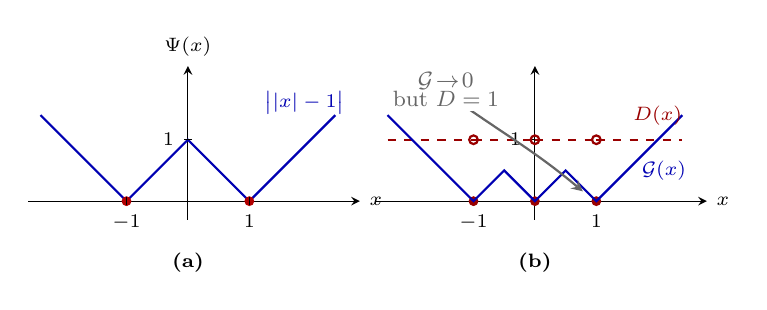
\begin{tikzpicture}[>=stealth, font=\scriptsize, scale=0.78]
 
% ================================================================
% Panel (a):  Psi(x) = ||x|-1|
% ================================================================
\begin{scope}[xshift=0cm]
 
  % axes
  \draw[->] (-2.6,0) -- (2.8,0) node[right] {$x$};
  \draw[->] (0,-0.3) -- (0,2.2) node[above] {$\Psi(x)$};
 
  % Psi(x) = ||x|-1|
  % key points: (-2,1) (-1,0) (0,1) (1,0) (2,1)
  \draw[thick, blue!70!black]
    (-2.4,1.4) -- (-1,0) -- (0,1) -- (1,0) -- (2.4,1.4);
 
  % mark minimizers
  \filldraw[red!70!black] (-1,0) circle (2pt);
  \filldraw[red!70!black] ( 1,0) circle (2pt);
 
  % tick marks
  \draw (-1,0.07) -- (-1,-0.07) node[below] {$-1$};
  \draw ( 1,0.07) -- ( 1,-0.07) node[below] {$1$};
  \draw (0.07,1) -- (-0.07,1) node[left] {$1$};
 
  % label
  \node[blue!70!black] at (1.9,1.6) {$\bigl||x|-1\bigr|$};
 
  % panel label
  \node at (0,-1.0) {\textbf{(a)}};
 
\end{scope}
 
% ================================================================
% Panel (b):  D(x) vs G(x)
% ================================================================
\begin{scope}[xshift=5.65cm]
 
  % axes
  \draw[->] (-2.6,0) -- (2.8,0) node[right] {$x$};
  \draw[->] (0,-0.3) -- (0,2.2);
 
  % tick marks
  \draw (-1,0.07) -- (-1,-0.07) node[below] {$-1$};
  \draw ( 1,0.07) -- ( 1,-0.07) node[below] {$1$};
  \draw (0.07,1) -- (-0.07,1) node[left] {$1$};
 
  % --- D(x): dashed, step function at 1, with jumps at {-1,0,1} ---
  \draw[thick, dashed, red!60!black]
    (-2.4,1) -- (-1,1);
  \draw[thick, dashed, red!60!black]
    (-1,1) -- (0,1);
  \draw[thick, dashed, red!60!black]
    (0,1) -- (1,1);
  \draw[thick, dashed, red!60!black]
    (1,1) -- (2.4,1);
 
  % open circles at D=1 for x in {-1,0,1}
  \draw[red!60!black, thick] (-1,1) circle (2pt);
  \draw[red!60!black, thick] ( 0,1) circle (2pt);
  \draw[red!60!black, thick] ( 1,1) circle (2pt);
 
  % closed circles at D=0 for x in {-1,0,1}
  \filldraw[red!60!black] (-1,0) circle (2pt);
  \filldraw[red!60!black] ( 0,0) circle (2pt);
  \filldraw[red!60!black] ( 1,0) circle (2pt);
 
  % --- G(x): solid, piecewise linear ---
  % G(x) = |x|              for 0<=|x|<=1/2
  %       = 1-|x|           for 1/2<=|x|<=1
  %       = |x|-1           for |x|>=1
  % key points: (-2,1) (-1,0) (-0.5,0.5) (0,0) (0.5,0.5) (1,0) (2,1)
  \draw[thick, blue!70!black]
    (-2.4,1.4) -- (-1,0) -- (-0.5,0.5) -- (0,0)
    -- (0.5,0.5) -- (1,0) -- (2.4,1.4);
 
  % labels
  \node[red!60!black]  at (2.0, 1.4) {$D(x)$};
  \node[blue!70!black] at (2.1, 0.5) {$\mathcal{G}(x)$};
 
  % annotation arrow: highlight the gap near x=1
  \draw[->, thick, black!60] (-1.25,1.62) to[out=-35,in=140] (0.78,0.16);
  \node[black!60, align=center, fill=white, inner sep=1.5pt]
    at (-1.45,1.82)
    {\footnotesize $\mathcal{G}\!\to\!0$\\[-1pt]\footnotesize but $D=1$};
 
  % panel label
  \node at (0,-1.0) {\textbf{(b)}};
 
\end{scope}
\end{tikzpicture}
\caption{Exact critical-distance residual versus Fenchel-gap behavior in the one-dimensional example.}
\label{fig:exact-vs-fenchel-gap}
\end{figure}

\begin{example}[Exact vs.\ Fenchel-gap certificate]
\label{ex:motivating-dc-gap}
Consider
\[
    \Psi(x)=\bigl||x|-1\bigr|
    =
    \phi(x)-g(x),
\]
where \( \phi(x)=3+4(|x|-1)_+ \) and \( g(x)=|x+1|+|x|+|x-1| \). Both \(\phi\) and \(g\) are convex, and \(g\) is nonsmooth at the global minimizers \(x=\pm1\). The exact same-point critical-distance residual is
\[
    D(x)
    :=
    \operatorname{dist}\bigl(0,\partial\phi(x)-\partial g(x)\bigr)
    =
    \begin{cases}
    0, & x\in\{-1,0,1\},\\
    1, & \text{otherwise}.
    \end{cases}
\]
Hence, even when \(x\) is arbitrarily close to the nonsmooth minimizer \(x=1\), the exact critical distance remains \(D(x)=1\).

For comparison, specialize the two-sided Fenchel certificate to the common-certificate scalar gap
\[
    \calG(x)
    :=
    \inf\limits_{b\in\RR}
    \left\{
        \Phi_\phi(x,b)+\Phi_g(x,b)
    \right\}.
\]
This corresponds to the case \(\bu=\bv=b\): the same scalar \(b\) must act as an approximate subgradient certificate for both convex components at the same point. A direct conjugate calculation gives
\[
\begin{aligned}
    \phi^*(b)
    &=
    \begin{cases}
        |b|-3, & |b|\le 4,\\
        +\infty, & |b|>4,
    \end{cases}
    \\
    g^*(b)
    &=
    \begin{cases}
        -2, & |b|\le 1,\\
        |b|-3, & 1\le |b|\le 3,\\
        +\infty, & |b|>3.
    \end{cases}
\end{aligned}
\]
Consequently,
\[
    \calG(x)
    =
    \begin{cases}
        |x|, & 0\le |x|\le \frac12,\\
        1-|x|, & \frac12\le |x|\le 1,\\
        |x|-1, & |x|\ge 1.
    \end{cases}
\]
In particular, \(\calG(x)\to0\) as \(x\to\pm1\), while \(D(x)=1\) for every \(x\notin\{-1,0,1\}\). Equivalently, near \(x=1\), choosing \(b=1\in\partial g(x)\) for \(0<x<1\) gives
\[
    \Phi_g(x,1)=0,
    \qquad
    \Phi_\phi(x,1)=1-x\to0
    \;\;\text{as }x\uparrow1,
\]
and choosing \(b=3\in\partial g(x)\) for \(x>1\) gives
\[
    \Phi_g(x,3)=0,
    \qquad
    \Phi_\phi(x,3)=x-1\to0
    \;\;\text{as }x\downarrow1.
\]
This is the behavior shown in \Cref{fig:exact-vs-fenchel-gap}: the Fenchel gap accurately detects convergence toward a nonsmooth minimizer, whereas the exact critical distance remains an \(O(1)\) step function around it.
\end{example}

\Cref{ex:motivating-dc-gap} shows that the $(\delta_\phi,\delta_g,\varepsilon)$-critical point repairs the diagnostic failure of the exact residual, but a diagnostic that is easy to satisfy is only useful if it is also sound: an overly permissive relaxation could remain satisfiable at points bearing no relation to criticality at all. We close this section by ruling out this concern as follows.
 The next proposition shows that \Cref{def:delta-eps-critical} degenerates correctly, in the sense that driving all three tolerances to zero forces exact DC criticality at the same point.
This properpsition depends on the monotonicity of the $\delta$-subdifferential in $\delta$ together with lower semicontinuity of $\phi,\phi^*,g,g^*$; 

\begin{proposition}
\label{prop:exact-consistency}
Suppose $\phi$ and $g$ are $G$-Lipschitz on $\RR^n$. If $\bar\bx$ is a $(\delta_\phi^{(k)},\delta_g^{(k)},\varepsilon^{(k)})$-critical point of Problem~\eqref{Eq: unconstrained DC problem} for every $k\in\NN$, with $\delta_\phi^{(k)},\delta_g^{(k)},\varepsilon^{(k)}\to0$ as $k\to\infty$, then $\bar\bx$ is a critical point of Problem~\eqref{Eq: unconstrained DC problem}, i.e., $\zero\in\partial\phi(\bar\bx)-\partial g(\bar\bx)$.
\end{proposition}

\begin{proof}
For each $k$, choose $\bu_k\in\partial_{\delta_\phi^{(k)}}\phi(\bar\bx)$ and $\bv_k\in\partial_{\delta_g^{(k)}}g(\bar\bx)$ with $\|\bu_k-\bv_k\|\le\varepsilon^{(k)}$. Since $\phi$ is $G$-Lipschitz on all of $\RR^n$, every element of $\partial_\delta\phi(\bar\bx)$ has norm at most $G$, regardless of $\delta$: for $\bv\in\partial_\delta\phi(\bar\bx)$, the defining inequality $\phi(\bar\bx)+G\|\bz-\bar\bx\|\ge\phi(\bz)\ge\phi(\bar\bx)+\langle\bv,\bz-\bar\bx\rangle-\delta$ along $\bz-\bar\bx=t\bv/\|\bv\|$ forces $\|\bv\|\le G+\delta/t$ for every $t>0$, hence $\|\bv\|\le G$ as $t\to\infty$. The same bound holds for $\partial_\delta g(\bar\bx)$. Thus $\{\bu_k\}$ and $\{\bv_k\}$ are bounded, and we may pass to a subsequence along which $\bu_k\to\bu^\star$ and $\bv_k\to\bv^\star$; since $\|\bu_k-\bv_k\|\to0$, we get $\bu^\star=\bv^\star=:\bw$.

It remains to show $\bw\in\partial\phi(\bar\bx)$; the argument for $\bw\in\partial g(\bar\bx)$ is identical. Since $\phi$ and $\phi^*$ are proper, closed, and convex, both are lower semicontinuous, so
\[
    \Phi_\phi(\bar\bx,\bw)
    =\phi(\bar\bx)+\phi^*(\bw)-\langle\bw,\bar\bx\rangle
    \le\liminf_{k\to\infty}\Bigl[\phi(\bar\bx)+\phi^*(\bu_k)-\langle\bu_k,\bar\bx\rangle\Bigr]
    =\liminf_{k\to\infty}\Phi_\phi(\bar\bx,\bu_k)
    \le\liminf_{k\to\infty}\delta_\phi^{(k)}=0.
\]
The Fenchel--Young inequality gives $\Phi_\phi(\bar\bx,\bw)\ge0$ unconditionally, so $\Phi_\phi(\bar\bx,\bw)=0$, i.e., $\bw\in\partial\phi(\bar\bx)$. Hence $\bw\in\partial\phi(\bar\bx)\cap\partial g(\bar\bx)$, and $\zero=\bw-\bw\in\partial\phi(\bar\bx)-\partial g(\bar\bx)$.
\end{proof}


% no spatial displacement argument is needed, since the collapse takes place at the fixed point $\bar\bx$. This is a first indication of a recurring theme in \Cref{sec:relationship-relaxed-dc-criticality} below: relaxing criticality along the value axis, rather than the spatial axis, tends to keep the base point fixed throughout.

\subsection{Relationship between Relaxed DC Criticality Notions}
\label{sec:relationship-relaxed-dc-criticality}

We show that the $(\delta_\phi,\delta_g,\varepsilon)$-critical point in
\Cref{def:delta-eps-critical} is a unifying value-relaxed formulation:
every previously proposed relaxed DC criticality notion for
Problem~\eqref{Eq: unconstrained DC problem} embeds into
\Cref{def:delta-eps-critical} for a suitable choice of
$(\delta_\phi,\delta_g,\varepsilon)$, and this embedding admits a sharper,
second-order accurate rate whenever the underlying component is smooth.

We recall three such notions, in increasing order of the spatial freedom
they allow.

\begin{definition}[$\varepsilon$-critical point~\citep{moudafi2021complete,sun2023algorithms}]
\label{Def: epsilon-critical point in DC}
Given $\varepsilon>0$, a point $\bar\bx\in\RR^n$ is an $\varepsilon$-critical
point of Problem~\eqref{Eq: unconstrained DC problem} if there exist
$\bar\by\in\RR^n$ and $\bar\bu\in\partial\phi(\bar\bx)-\partial g(\bar\by)$
such that
\[
    \max\limits\{\|\bar\bu\|,\|\bar\bx-\bar\by\|\}\le\varepsilon .
\]
\end{definition}

\begin{definition}[Nearly $\varepsilon$-critical point~\citep{yao2022large}]
\label{Def: epsilon-critical point 3}
Given $\varepsilon>0$, a point $\bar\bx\in\RR^n$ is a nearly
$\varepsilon$-critical point of Problem~\eqref{Eq: unconstrained DC problem}
if there exist $\bar\by_1,\bar\by_2\in\RR^n$ and
$\bar\bu\in\partial\phi(\bar\by_1)-\partial g(\bar\by_2)$ such that
\[
    \max\limits\{\|\bar\bu\|,\|\bar\bx-\bar\by_1\|,\|\bar\bx-\bar\by_2\|\}
    \le\varepsilon .
\]
\end{definition}

\begin{definition}[Nearly $\varepsilon$-stationary point~\citep{xu2019stochastic}]
\label{def:xu-near-stationary}
Given $\varepsilon>0$, a point $\bar\bx\in\RR^n$ is a nearly
$\varepsilon$-stationary point of Problem~\eqref{Eq: unconstrained DC
problem} if there exist $c>0$ and $\bx^*\in\RR^n$ with
$\|\bar\bx-\bx^*\|\le c\varepsilon$ such that
\[
    \operatorname{dist}\bigl(\partial\phi(\bx^*),\partial g(\bx^*)\bigr)
    \le\varepsilon .
\]
\end{definition}

Definitions~\ref{Def: epsilon-critical point in DC} and
\ref{Def: epsilon-critical point 3} relax criticality by letting $\phi$
and $g$ be evaluated at points that may drift apart from each other and
from $\bar\bx$; \Cref{def:xu-near-stationary} instead forces $\phi$ and
$g$ to share a common witness point $\bx^*$, which itself may drift from
$\bar\bx$. All three reduce to a single mechanism: converting a spatial
offset into a Fenchel-gap slack.

\begin{lemma}
\label{lem:spatial-to-value}
Let $q:\RR^n\to\RR\cup\{+\infty\}$ be proper, closed, convex, and
$G$-Lipschitz on a convex set containing $\bx,\by\in\operatorname{dom}q$.
\begin{enumerate}
    \item[(a)] If $\bv\in\partial q(\by)$, then
    $\bv\in\partial_{2G\|\bx-\by\|}q(\bx)$.
    \item[(b)] If, in addition, $q$ is $L$-smooth on this set and
    $\bv=\nabla q(\by)$, then
    $\bv\in\partial_{\frac{L}{2}\|\bx-\by\|^2}q(\bx)$.
\end{enumerate}
\end{lemma}

\begin{proof}
By the Fenchel--Young equality at a subgradient,
$q^*(\bv)=\langle\bv,\by\rangle-q(\by)$, so
\[
    \Phi_q(\bx,\bv)
    = q(\bx)-q(\by)-\langle\bv,\bx-\by\rangle
    =: D_q(\bx,\by).
\]
(a) Convexity gives $D_q(\bx,\by)\ge0$; $G$-Lipschitzness gives
$q(\bx)-q(\by)\le G\|\bx-\by\|$ and $\|\bv\|\le G$, so
$D_q(\bx,\by)\le 2G\|\bx-\by\|$.
(b) $D_q(\bx,\by)$ is the Bregman divergence of $q$ at $(\bx,\by)$; for
convex $L$-smooth $q$ it satisfies $0\le D_q(\bx,\by)\le\tfrac
L2\|\bx-\by\|^2$ by the descent lemma.
\end{proof}
We then establish that the $(\delta_\phi,\delta_g,\varepsilon)$-critical point in \Cref{def:delta-eps-critical} recovers all three existing relaxed DC criticality notions
\begin{proposition}
\label{prop:recovery-existing-dc-criticality}
Suppose $\phi$ and $g$ are, respectively, $G_\phi$- and $G_g$-Lipschitz on
the relevant neighborhoods below. Then:
\begin{enumerate}
    \item[(i)] If $\bar\bx$ is an $\varepsilon$-critical point in the
    sense of \Cref{Def: epsilon-critical point in DC}, then $\bar\bx$ is a
    $(0,\,2G_g\varepsilon,\,\varepsilon)$-critical point.
    \item[(ii)] If $\bar\bx$ is a nearly $\varepsilon$-critical point in
    the sense of \Cref{Def: epsilon-critical point 3}, then $\bar\bx$ is a
    $(2G_\phi\varepsilon,\,2G_g\varepsilon,\,\varepsilon)$-critical point.
    \item[(iii)] If $\bar\bx$ is a nearly $\varepsilon$-stationary point in
    the sense of \Cref{def:xu-near-stationary}, then $\bar\bx$ is a
    $(2G_\phi c\varepsilon,\,2G_g c\varepsilon,\,\varepsilon)$-critical
    point.
\end{enumerate}
\end{proposition}

\begin{proof}
(i) Write $\bar\bu=\bp-\bq$ with $\bp\in\partial\phi(\bar\bx)
=\partial_0\phi(\bar\bx)$ and $\bq\in\partial g(\bar\by)$.
\Cref{lem:spatial-to-value}(a) with $q=g$, $\bx=\bar\bx$, $\by=\bar\by$
gives $\bq\in\partial_{2G_g\|\bar\bx-\bar\by\|}g(\bar\bx)\subseteq
\partial_{2G_g\varepsilon}g(\bar\bx)$, so
$\operatorname{dist}(\partial_0\phi(\bar\bx),\partial_{2G_g\varepsilon}g(\bar\bx))
\le\|\bp-\bq\|=\|\bar\bu\|\le\varepsilon$.

(ii) Identical, applying \Cref{lem:spatial-to-value}(a) to both
$\bp\in\partial\phi(\bar\by_1)$ and $\bq\in\partial g(\bar\by_2)$.

(iii) Take $\bp\in\partial\phi(\bx^*)$, $\bq\in\partial g(\bx^*)$ with
$\|\bp-\bq\|\le\varepsilon$; this is exactly case (ii) with
$\bar\by_1=\bar\by_2=\bx^*$ and spatial offset $c\varepsilon$ in place of
$\varepsilon$.
\end{proof}

\begin{remark}
Case (iii) is not an independent construction: it is case (ii)
specialized to a common witness point. The distinction between
\Cref{Def: epsilon-critical point in DC}/\ref{Def: epsilon-critical point 3}
and \Cref{def:xu-near-stationary} is therefore not a difference in the
relaxation mechanism, but only in whether the two witness points are
allowed to coincide.
\end{remark}

The embedding above only uses Lipschitz continuity and is tight up to
constants. When a component happens to be smooth,
\Cref{lem:spatial-to-value}(b) applies in place of (a) and yields a
second-order accurate slack on that side.

\begin{proposition}
\label{prop:sharp-smooth}
In the setting of \Cref{def:xu-near-stationary}, suppose in addition that
$g$ is convex and $L_g$-smooth on a neighborhood of $\bx^*$. Then
$\bar\bx$ is a
\[
    \Bigl(2G_\phi c\varepsilon,\ \tfrac{L_g}{2}c^2\varepsilon^2,\
    \varepsilon\Bigr)\text{-critical point}.
\]
If $\phi$ is also convex and $L_\phi$-smooth on a neighborhood of
$\bx^*$, the first slack sharpens to $\tfrac{L_\phi}{2}c^2\varepsilon^2$,
so that $\bar\bx$ is an
$\bigl(\mathcal O(\varepsilon^2),\,\mathcal O(\varepsilon^2),\,
\varepsilon\bigr)$-critical point.
\end{proposition}

\begin{proof}
Take $\bv^*=\nabla g(\bx^*)$ in place of an arbitrary
$\bq\in\partial g(\bx^*)$ in the proof of
\Cref{prop:recovery-existing-dc-criticality}(iii), and apply
\Cref{lem:spatial-to-value}(b) instead of (a):
$\bv^*\in\partial_{\frac{L_g}{2}\|\bar\bx-\bx^*\|^2}g(\bar\bx)
\subseteq\partial_{\frac{L_g}{2}c^2\varepsilon^2}g(\bar\bx)$. The
$\phi$-side bound is unchanged from
\Cref{prop:recovery-existing-dc-criticality}(iii). The refinement when
$\phi$ is also smooth follows by the same substitution on the
$\phi$-side.
\end{proof}

\Cref{prop:recovery-existing-dc-criticality} and
\Cref{prop:sharp-smooth} together show that
\Cref{def:delta-eps-critical} strictly subsumes
Definitions~\ref{Def: epsilon-critical point in DC},
\ref{Def: epsilon-critical point 3}, and \ref{def:xu-near-stationary}: the
value slack incurred is $\mathcal O(\varepsilon)$ under Lipschitz
continuity alone, and tightens to $\mathcal O(\varepsilon^2)$ on any
component that is additionally smooth. This also isolates precisely what
smoothness of $g$ buys in \citet{xu2019stochastic}: it is not needed for
the embedding into \Cref{def:delta-eps-critical}, which only requires
Lipschitz continuity, but it tightens the resulting slack by one order in
$\varepsilon$.

\subsubsection{The Converse Embedding}

\Cref{prop:recovery-existing-dc-criticality} and \Cref{prop:sharp-smooth}
show that $(\delta_\phi,\delta_g,\varepsilon)$-criticality is no harder to
satisfy than any previously proposed relaxed DC criticality notion. We now
establish the converse direction: satisfying \Cref{def:delta-eps-critical}
is also no easier, in the sense that it forces the same qualitative
conclusion as \Cref{Def: epsilon-critical point 3}, up to an explicit loss
of one order in the tolerance. The mechanism is the classical reachback
theorem of Brøndsted and Rockafellar~\citep{brondsted1965subdifferentiability},
which converts an approximate subgradient at $\bar\bx$ into an exact
subgradient at a nearby point, and is the exact converse of
\Cref{lem:spatial-to-value}(a).

\begin{lemma}
\label{lem:value-to-spatial}
Let $q:\RR^n\to\RR\cup\{+\infty\}$ be proper, closed, and convex, and let
$\bv\in\partial_\delta q(\bar\bx)$ for some $\delta>0$. Then for every
$\lambda>0$ there exist $\hat\bx\in\RR^n$ and $\hat\bv\in\partial
q(\hat\bx)$ such that
\[
    \|\hat\bx-\bar\bx\|\le\lambda,
    \qquad
    \|\hat\bv-\bv\|\le\frac{\delta}{\lambda}.
\]
In particular, taking $\lambda=\sqrt\delta$ gives
$\|\hat\bx-\bar\bx\|\le\sqrt\delta$ and $\|\hat\bv-\bv\|\le\sqrt\delta$.
\end{lemma}

\begin{proposition}[Reverse embedding]
\label{prop:reverse-embedding}
If $\bar\bx$ is a $(\delta_\phi,\delta_g,\varepsilon)$-critical point of
Problem~\eqref{Eq: unconstrained DC problem}, then $\bar\bx$ is a nearly
$\varepsilon'$-critical point in the sense of
\Cref{Def: epsilon-critical point 3}, with
\[
    \varepsilon'=\varepsilon+\sqrt{\delta_\phi}+\sqrt{\delta_g}.
\]
\end{proposition}

\begin{proof}
Let $\bu\in\partial_{\delta_\phi}\phi(\bar\bx)$ and
$\bv\in\partial_{\delta_g}g(\bar\bx)$ with $\|\bu-\bv\|\le\varepsilon$.
Apply \Cref{lem:value-to-spatial} to $\bu$ with $\lambda=\sqrt{\delta_\phi}$
and to $\bv$ with $\lambda=\sqrt{\delta_g}$, obtaining $\bar\by_1$,
$\hat\bu\in\partial\phi(\bar\by_1)$ and $\bar\by_2$,
$\hat\bv\in\partial g(\bar\by_2)$ with $\|\bar\by_1-\bar\bx\|\le\sqrt{\delta_\phi}$,
$\|\hat\bu-\bu\|\le\sqrt{\delta_\phi}$, and analogously for
$\bar\by_2,\hat\bv$. Set $\bar\bu:=\hat\bu-\hat\bv\in\partial\phi(\bar\by_1)-\partial g(\bar\by_2)$. The triangle inequality gives
\[
    \|\bar\bu\|
    \le\|\hat\bu-\bu\|+\|\bu-\bv\|+\|\bv-\hat\bv\|
    \le\sqrt{\delta_\phi}+\varepsilon+\sqrt{\delta_g}=\varepsilon',
\]
while $\|\bar\bx-\bar\by_1\|\le\sqrt{\delta_\phi}\le\varepsilon'$ and
$\|\bar\bx-\bar\by_2\|\le\sqrt{\delta_g}\le\varepsilon'$, which verifies the
defining condition of \Cref{Def: epsilon-critical point 3} with
$\varepsilon'$ in place of $\varepsilon$.
\end{proof}

\begin{proposition}[Same-point refinement under smoothness]
\label{prop:reverse-smooth}
In the setting of \Cref{prop:reverse-embedding}, suppose in addition that
$g$ is convex and $L_g$-smooth on a neighborhood of $\bar\bx$. Then
\[
    \operatorname{dist}\bigl(\nabla g(\bar\bx),\,\partial_{\delta_\phi}\phi(\bar\bx)\bigr)
    \le\varepsilon+\sqrt{2L_g\delta_g}.
\]
If $\phi$ is also convex and $L_\phi$-smooth on a neighborhood of
$\bar\bx$, then
\[
    \bigl\|\nabla\phi(\bar\bx)-\nabla g(\bar\bx)\bigr\|
    \le\varepsilon+\sqrt{2L_\phi\delta_\phi}+\sqrt{2L_g\delta_g},
\]
so that $\bar\bx$ is, up to this explicit slack, a same-point approximate
stationary point of the smooth DC problem.
\end{proposition}

\begin{proof}
For $L_g$-smooth convex $g$, the conjugate $g^*$ is
$\tfrac1{L_g}$-strongly convex, so $\Phi_g(\bar\bx,\bv)\ge
\tfrac1{2L_g}\|\bv-\nabla g(\bar\bx)\|^2$ for every $\bv$. Applied to
$\bv\in\partial_{\delta_g}g(\bar\bx)$, this gives
$\|\bv-\nabla g(\bar\bx)\|\le\sqrt{2L_g\delta_g}$; combined with
$\bu\in\partial_{\delta_\phi}\phi(\bar\bx)$ and $\|\bu-\bv\|\le\varepsilon$,
the triangle inequality gives the first bound. The second bound follows by
the same argument applied to $\bu$ once $\phi$ is also $L_\phi$-smooth and
convex.
\end{proof}

\begin{remark}[Asymmetry between the two directions]
The two directions are not symmetric. Embedding an existing notion into
\Cref{def:delta-eps-critical} costs a value slack linear in the spatial
tolerance under Lipschitz continuity alone (\Cref{lem:spatial-to-value}(a))
and quadratic under smoothness (\Cref{lem:spatial-to-value}(b)). Recovering
an existing notion from \Cref{def:delta-eps-critical} costs a spatial
displacement on the order of the square root of the value tolerance under
Lipschitz continuity alone (\Cref{lem:value-to-spatial}); this square-root
rate is the classical Brøndsted--Rockafellar rate and is not, in general,
improvable to a linear one. Smoothness removes the asymmetry in the
strongest sense: on a smooth component, the reverse direction also
collapses to a same-point bound (\Cref{prop:reverse-smooth}), matching the
same-point character of the forward direction under smoothness
(\Cref{prop:sharp-smooth}), at the cost of a square-root rather than a
quadratic rate.
\end{remark}

\subsubsection{Relation to Goldstein Stationarity}

We conclude by relating $(\delta_\phi,\delta_g,\varepsilon)$-criticality to
a relaxed stationarity notion outside the DC literature: the Goldstein
$\delta$-subdifferential relaxation of Clarke stationarity
\citep{goldstein1977optimization,Zhang-2020-Complexity}, introduced
schematically in \Cref{fig:goldstein-vs-approximate-subdifferential}. For a
locally Lipschitz function $F:\RR^n\to\RR$, the Goldstein
$\delta$-subdifferential at $\bar\bx$ is
\[
    \partial_\delta^G F(\bar\bx)
    :=
    \overline{\operatorname{conv}}
    \bigcup_{\by\in B_\delta(\bar\bx)}
    \partial_C F(\by),
\]
and $\bar\bx$ is a $(\delta,\varepsilon)$-Goldstein stationary point of $F$
if $\operatorname{dist}(\zero,\partial_\delta^G F(\bar\bx))\le\varepsilon$,
where $B_\delta(\bar\bx):=\{\by\in\RR^n:\|\by-\bar\bx\|\le\delta\}$.
Applied to $F=\Psi=\phi-g$, this relaxes Clarke stationarity along the
spatial axis: it collects exact generalized gradients over a
$\delta$-neighborhood of $\bar\bx$ and convexifies, rather than relaxing
the defining inequality at $\bar\bx$ itself. \Cref{def:delta-eps-critical}
relaxes along the orthogonal, value axis, and couples $\phi$ and $g$
independently rather than through a common witness point in
$B_\delta(\bar\bx)$. \Cref{tab:goldstein-vs-ours} summarizes the
distinction.

\begin{table}[t]
\centering
\caption{Two relaxation mechanisms for the same base criterion
$\zero\in\partial\phi(\bar\bx)-\partial g(\bar\bx)$.}
\label{tab:goldstein-vs-ours}
\small
\begin{tabular}{lll}
\hline
 & $(\delta,\varepsilon)$-Goldstein & $(\delta_\phi,\delta_g,\varepsilon)$-critical \\
\hline
Relaxation axis & spatial, $B_\delta(\bar\bx)$ & value, Fenchel--Young gap \\
Witness structure & common $\by\in B_\delta(\bar\bx)$ & independent $\bu,\bv$ at $\bar\bx$ \\
Evaluation point & nearby $\by$ & $\bar\bx$ itself \\
\hline
\end{tabular}
\end{table}

Despite this structural difference, the Goldstein relaxation embeds into
ours.

\begin{lemma}[Goldstein bridge]
\label{cor:goldstein-bridge}
Let $q:\RR^n\to\RR\cup\{+\infty\}$ be proper, closed, convex, and
$G$-Lipschitz on a convex set containing $B_\delta(\bar\bx)$. Then
\[
    \bigcup_{\by\in B_\delta(\bar\bx)}\partial q(\by)
    \subseteq
    \partial_{2G\delta}q(\bar\bx).
\]
\end{lemma}

\begin{proof}
Immediate from \Cref{lem:spatial-to-value}(a): for $\by\in B_\delta(\bar\bx)$
and $\bv\in\partial q(\by)$, $\|\bar\bx-\by\|\le\delta$ gives
$\bv\in\partial_{2G\delta}q(\bar\bx)$.
\end{proof}

\begin{proposition}[Goldstein implies ours]
\label{prop:goldstein-implies-ours}
Suppose $\phi,g$ are, respectively, $G_\phi$- and $G_g$-Lipschitz on a
convex set containing $B_\delta(\bar\bx)$. If $\bar\bx$ is a
$(\delta,\varepsilon)$-Goldstein stationary point of $\Psi=\phi-g$, then
$\bar\bx$ is a $(2G_\phi\delta,\,2G_g\delta,\,\varepsilon)$-critical point.
\end{proposition}

\begin{proof}
Let $\bw\in\partial_\delta^G\Psi(\bar\bx)$ with $\|\bw\|\le\varepsilon$. By
Carath\'eodory's theorem, $\bw=\sum_i\lambda_i\bw_i$ for finitely many
$\bw_i\in\partial_C\Psi(\by_i)$, $\by_i\in B_\delta(\bar\bx)$,
$\lambda_i\ge0$, $\sum_i\lambda_i=1$. By the Clarke sum rule for the
difference of two convex functions, $\bw_i=\bu_i-\bv_i$ with
$\bu_i\in\partial\phi(\by_i)$, $\bv_i\in\partial g(\by_i)$. Set
$\bar\bu:=\sum_i\lambda_i\bu_i$ and $\bar\bv:=\sum_i\lambda_i\bv_i$. By
\Cref{cor:goldstein-bridge}, each $\bu_i\in\partial_{2G_\phi\delta}\phi(\bar\bx)$;
since $\partial_{2G_\phi\delta}\phi(\bar\bx)$ is an intersection of
half-spaces, it is convex, so $\bar\bu\in\partial_{2G_\phi\delta}\phi(\bar\bx)$.
Likewise $\bar\bv\in\partial_{2G_g\delta}g(\bar\bx)$. Since
$\bar\bu-\bar\bv=\sum_i\lambda_i\bw_i=\bw$,
\[
    \operatorname{dist}\bigl(\partial_{2G_\phi\delta}\phi(\bar\bx),\partial_{2G_g\delta}g(\bar\bx)\bigr)
    \le\|\bar\bu-\bar\bv\|=\|\bw\|\le\varepsilon.
    \qedhere
\]
\end{proof}

The converse fails in general, and the reason is structural rather than a
looseness of constants: the DC decomposition can manufacture a critical
point that $\Psi$ itself does not have.

\begin{example}[The converse fails]
\label{ex:goldstein-counterexample}
Let $\phi(x)=\max\limits(x,0)$ and $g(x)=\max\limits(-x,0)$ on $\RR$, and consider
$\bar x=0$. Then $\partial\phi(0)=[0,1]$ and $\partial g(0)=[-1,0]$, so
$\partial\phi(0)-\partial g(0)=[0,2]\ni0$: $\bar x=0$ is an exact DC
critical point, i.e., a $(0,0,0)$-critical point. However,
$\Psi(x)=\phi(x)-g(x)=x$ for every $x$, so $\partial_C\Psi\equiv\{1\}$
everywhere, and $\partial_\delta^G\Psi(0)=\{1\}$ for every $\delta\ge0$.
Hence $\operatorname{dist}(0,\partial_\delta^G\Psi(0))=1$ for every
$\delta\ge0$, and $\bar x=0$ is never a $(\delta,\varepsilon)$-Goldstein
stationary point for $\varepsilon<1$.
\end{example}

\begin{remark}[Agreement under a faithful decomposition]
\label{rem:faithful-decomposition}
\blue{If $\phi$ is differentiable at $\bar\bx$, the Clarke sum rule holds with
equality,
\[
    \partial_C\Psi(\bar\bx)=\nabla\phi(\bar\bx)-\partial g(\bar\bx)=\partial\phi(\bar\bx)-\partial g(\bar\bx),
\]
and symmetrically if $g$ is differentiable at $\bar\bx$.} We call such a
decomposition \emph{faithful} at $\bar\bx$: exact DC criticality and exact
Clarke stationarity of $\Psi$ coincide there, so the inflation exhibited in
\Cref{ex:goldstein-counterexample} cannot occur. That example is unfaithful
precisely because $\phi$ and $g$ are simultaneously nonsmooth at
$\bar x=0$; nonsmoothness on at most one side already rules it out.
\end{remark}

Taken together,
\Cref{prop:recovery-existing-dc-criticality,prop:sharp-smooth,prop:reverse-embedding,prop:reverse-smooth,prop:goldstein-implies-ours}
position $(\delta_\phi,\delta_g,\varepsilon)$-criticality against every
relaxed stationarity notion available in the DC and nonsmooth nonconvex
literature: it is implied by each of them under Lipschitz continuity
alone, it implies a matching notion in return at the cost of a
square-root loss inherent to reachback from a value relaxation, and both
directions tighten to a same-point bound whenever the relevant component
is smooth. \Cref{ex:goldstein-counterexample} shows that the reverse
implication from Goldstein stationarity cannot be strengthened to an
equivalence without restricting to faithful decompositions, an intrinsic
limitation of relaxing criticality at the level of a DC pair rather than
at the level of $\Psi$ itself.

\section{Complexity Analysis of DCA}
\label{sec:complexity-analysis-DCA}
\begin{algorithm}[tbp]
    \caption{\textbf{(In)exact DCA}}
    \label{alg: DCA}
    \begin{algorithmic}[1]
        \STATE {\bfseries Input:} Initial point $\bx^0\in\dom \phi $,
        inner solver tolerance $\{\epsilon_k\}_{k=0}^{K-1}$,
        stepsize $\eta$.
        \FOR{$k=0,1,\ldots,K-1$}
            \STATE Compute $\bv^k \in \partial g(\bx^k)$.
            \STATE 
            Solve inner strongly convex subproblem:

            \STATE $\triangleright$ \textbf{Option I:} exact subproblem solve
            \begin{align}
            \label{eq:dca-exact-step}
            \bx^{k+1} = \argmin\limits_{\bx \in \RR^n } \{ \phi (\bx)- \langle \bv^k, \bx \rangle \} 
            \end{align}

            \STATE $\triangleright$ \textbf{Option II:} inexact inner solve
            \begin{align}
            \label{eq:dca-inner-solver-step}
            \bx^{k+1}
            =
            \mathcal S_{\mathcal A_k}(\bx^k,\bv^k;\Theta_k),
            \end{align}
            where $\mathcal S_{\mathcal A_k}$ denotes the inner solver selected
            by $\mathcal A_k$, and $\Theta_k$ collects its parameters and
            stopping tolerance.
        \ENDFOR
        \STATE {\bfseries Output:} $\hat\bx$, chosen uniformly from
        $\{\bx^k\}_{k=0}^{K-1}$.
    \end{algorithmic}
\end{algorithm} 

We use the unified DCA summarized in Algorithm~\ref{alg: DCA}. At the
$k$-th iteration, DCA computes a subgradient $\bv^k \in \partial g(\bx^k)$
and solves a $\gamma$-strongly convex subproblem to obtain $\bx^{k+1}$
(Option I). Option II is an abstract inexact inner-solver interface:
the proximal-subgradient method in
Algorithm~\ref{alg:prox-subgrad-dca-inner} is one realization, and other
inner-loop algorithms can be used as long as their output satisfies the
inexact certificate required in the analysis below.

Before analyzing the complexity of DCA, we first introduce the main
assumptions used throughout the section.

\subsection{Main Assumption}
Assume that $F$ is bounded below on $\operatorname{dom}\phi$, and denote
\[
F^\star:=\inf\limits_x F(x)>-\infty,
\qquad
\Delta_0:=F(\bx^0)-F^\star > 0.
\]
For any $\gamma>0$, $F$ admits the reformulation
\[
F = \Big(\phi+\tfrac{\gamma}{2}\|\bx\|^2\Big) - \Big(\tfrac{\gamma}{2}\|\bx\|^2+g\Big),
\]
so WLOG we take $\phi$ and $g$ to be $\gamma$-strongly convex, formalized as follows.

\begin{assumption}
\label{ass:strong-convexity-dc}
The functions $\phi$ and $g$ are strongly convex for some constant
$\gamma>0$, and $g$ has bounded subgradients:
$\sup\limits_{\bx}\sup\limits_{\bv\in\partial g(\bx)}\|\bv\|\le G$.
\end{assumption}

% We also take $\Delta_0>0$ WLOG: if $\Delta_0=0$, then $\bx^0$ is a global
% minimizer of $F$, so for any $\bv\in\partial g(\bx^0)$ and all $\bx$,
% \[
%     \phi(\bx)
%     \;\ge\;
%     g(\bx)+F(\bx^0)
%     \;\ge\;
%     g(\bx^0)+\langle\bv,\bx-\bx^0\rangle+F(\bx^0)
%     \;=\;
%     \phi(\bx^0)+\langle\bv,\bx-\bx^0\rangle,
% \]
% i.e., $\bv\in\partial\phi(\bx^0)\cap\partial g(\bx^0)$, so $\bx^0$ is already
% $(0,0,0)$-critical and the analysis is vacuous.
Our goal is to characterize the iteration complexity of DCA-type methods, without imposing smoothness on $g$, for reaching a $(\delta_\phi,\delta_g,\varepsilon)$-critical
point. As dicussed below, Tthe three parameters play distinct roles in this analysis:
$\varepsilon$ controls the residual mismatch between the approximate dual
vectors of $\phi$ and $g$, while $\delta_\phi$ and $\delta_g$ control how
loosely each convex component's Fenchel--Young gap is allowed to vanish.

\subsection{Common Auxilary Lemmas}
% In particular, $\delta_\phi$ coincides with the primal optimality gap of the
% convex subproblem solved at each DCA iteration,
% \[
%     \min\limits_{\bx}\ \phi(\bx)-\langle \bv^k,\bx\rangle,
% \]
% evaluated at the returned iterate $\bx^{k+1}$. If the subproblem is solved to
% global optimality (an exact oracle), then $\Phi_\phi(\bx^{k+1},\bv^k)=0$,
% i.e., $\delta_\phi=0$; if it is solved only approximately -- e.g., by a fixed
% budget of inner first-order steps -- then $\delta_\phi>0$, and its magnitude
% is precisely the residual primal gap left by the inner solver. Exact
% subproblem solution therefore recovers the stronger regime $\delta_\phi=0$,
% in which $\delta_g$ remains the only source of inexactness, reflecting its
% structural rather than computational origin.

The next lemma is the pivot of the analysis, which shows that the $\phi$-side Fenchel gap $\Phi_\phi$ is at any candidate point equals the value suboptimality of that
point for the current convex subproblem. Consequently, the parameter
$\delta_\phi$ of \Cref{def:delta-eps-critical} coincides, exactly and
without slack, with the accuracy to which the subproblem is solved.

\begin{lemma}
\label{lem:dca-subproblem-value}
Let \Cref{ass:strong-convexity-dc} hold, $\bar\bx\in\dom\phi$,
$\bv\in\partial g(\bar\bx)$, and define
$P(\bx):=\phi(\bx)-\langle\bv,\bx\rangle$. Then the following statements
hold.
\begin{enumerate}
    \item[(i)] $\inf\limits_{\bx\in\RR^n}P(\bx)\ge
    F^\ast+g(\bar\bx)-\langle\bv,\bar\bx\rangle>-\infty$, and
    $\phi^*(\bv)=-\inf\limits_{\bx\in\RR^n}P(\bx)\in\RR$.
    \item[(ii)] For every $\by\in\dom\phi$, the following holds
    \[
        \Phi_\phi(\by,\bv)
        \;=\;
        P(\by)-\inf\limits_{\bx\in\RR^n}P(\bx).
    \]
    \item[(iii)] For every $\sigma\ge0$ and every $\by\in\dom\phi$, the
    following three statements are equivalent:
    \[
        \text{(a) }P(\by)\le\inf\limits_{\bx\in\RR^n}P(\bx)+\sigma;
        \qquad
        \text{(b) }\Phi_\phi(\by,\bv)\le\sigma;
        \qquad
        \text{(c) }\bv\in\partial_\sigma\phi(\by).
    \]
    In particular, $\by\in\argmin\limits_{\bx\in\RR^n}P(\bx)$ if and only if
    $\bv\in\partial\phi(\by)$.
\end{enumerate}
\end{lemma}

\begin{proof}
(i) Since $\bar\bx\in\dom\phi\subseteq\dom g$ and
$\bv\in\partial g(\bar\bx)$, the subgradient inequality gives
\begin{equation}
    g(\bx)\;\ge\;g(\bar\bx)+\langle\bv,\bx-\bar\bx\rangle
    \qquad\text{for all }\bx\in\RR^n,
    \label{eq:g-subgrad-at-xbar}
\end{equation}
equivalently
$\langle\bv,\bx\rangle\le g(\bx)-g(\bar\bx)+\langle\bv,\bar\bx\rangle$
for all $\bx\in\RR^n$. Hence, for every $\bx\in\dom\phi\subseteq\dom g$,
\[
    P(\bx)
    \;=\;
    \phi(\bx)-\langle\bv,\bx\rangle
    \;\ge\;
    \phi(\bx)-g(\bx)+g(\bar\bx)-\langle\bv,\bar\bx\rangle
    \;=\;
    F(\bx)+g(\bar\bx)-\langle\bv,\bar\bx\rangle
    \;\ge\;
    F^\ast+g(\bar\bx)-\langle\bv,\bar\bx\rangle,
\]
while $P(\bx)=+\infty$ for $\bx\notin\dom\phi$. Since $g(\bar\bx)\in\RR$,
the claimed lower bound follows, and it is finite. Furthermore,
$P(\bar\bx)=\phi(\bar\bx)-\langle\bv,\bar\bx\rangle<+\infty$, so
$\inf\limits P\in\RR$. By the definition of the Fenchel conjugate,
\[
    \phi^*(\bv)
    \;=\;
    \sup\limits_{\bx\in\RR^n}\bigl\{\langle\bv,\bx\rangle-\phi(\bx)\bigr\}
    \;=\;
    -\inf\limits_{\bx\in\RR^n}\bigl\{\phi(\bx)-\langle\bv,\bx\rangle\bigr\}
    \;=\;
    -\inf\limits_{\bx\in\RR^n}P(\bx)\;\in\;\RR .
\]

(ii) For $\by\in\dom\phi$, using (i),
\[
    \Phi_\phi(\by,\bv)
    \;=\;
    \phi(\by)+\phi^*(\bv)-\langle\bv,\by\rangle
    \;=\;
    P(\by)+\phi^*(\bv)
    \;=\;
    P(\by)-\inf\limits_{\bx\in\RR^n}P(\bx).
\]

(iii) The equivalence of (a) and (b) is immediate from (ii). The
equivalence of (b) and (c) is \Cref{lem:fenchel-gap-toolkit} applied to
$h=\phi$. The final claim is the case $\sigma=0$.
\end{proof}


The following identity decomposes the per-iteration decrease of $F$
into three nonnegative quantities that together constitute a
$(\delta_\phi,\delta_g,\eps)$-point. It holds for an arbitrary
candidate $\bx^{k+1}$, regardless of how it is produced, and therefore
serves as the common engine underlying both the exact and the
inexact analyses.

\begin{lemma}[One-step decomposition identity]
\label{lem:dca-one-step-identity}
Suppose \Cref{ass:strong-convexity-dc} holds. For any
$\bx^k,\bx^{k+1}\in\dom\phi$ and any $\bv^k\in\partial g(\bx^k)$, it holds that
\begin{equation}
    F(\bx^{k+1})-F(\bx^k)
    \;=\;
    \Phi_\phi(\bx^{k+1},\bv^k)
    \;-\;
    \Phi_\phi(\bx^k,\bv^k)
    \;-\;
    \Phi_g(\bx^{k+1},\bv^k).
    \label{eq:dca-one-step-identity}
\end{equation}
% where
% \[
%     \Phi_\phi(\bx^k,\bv^k)\ge0,
%     \qquad
%     \Phi_\phi(\bx^{k+1},\bv^k)\ge0,
%     \qquad
%     \Phi_g(\bx^{k+1},\bv^k)\ge0.
% \]
\end{lemma}

\begin{proof}
By the Fenchel--Young equality, i.e.,  for any 
\begin{equation}
    g^*(\bv^k)
    \;=\;
    \langle\bv^k,\bx^k\rangle-g(\bx^k)
    \;\in\;\RR,
    \label{eq:fenchel-young-equality-g}
\end{equation} and 
ssubstituting \eqref{eq:fenchel-young-equality-g} into the definition of
$\Phi_g$ gives
\begin{equation}
    \Phi_g(\bx^{k+1},\bv^k)
    \;=\;
    g(\bx^{k+1})+g^*(\bv^k)-\langle\bv^k,\bx^{k+1}\rangle
    \;=\;
    g(\bx^{k+1})-g(\bx^k)-\langle\bv^k,\bx^{k+1}-\bx^k\rangle.
    \label{eq:g-gap-bregman-form}
\end{equation}

On the other hand, rearranging the terms in the definition of
$\Phi_\phi$ yields
\[
    \Phi_\phi(\bx^k,\bv^k)-\Phi_\phi(\bx^{k+1},\bv^k)
    \;=\;
    \bigl[\phi(\bx^k)-\langle\bv^k,\bx^k\rangle\bigr]
    -\bigl[\phi(\bx^{k+1})-\langle\bv^k,\bx^{k+1}\rangle\bigr].
\]

Adding \eqref{eq:g-gap-bregman-form} to the above equality yields
\[
    \Phi_\phi(\bx^k,\bv^k)-\Phi_\phi(\bx^{k+1},\bv^k)
    +\Phi_g(\bx^{k+1},\bv^k)
    \;=\;
    \bigl[\phi(\bx^k)-g(\bx^k)\bigr]
    -\bigl[\phi(\bx^{k+1})-g(\bx^{k+1})\bigr]
    \;=\;
    F(\bx^k)-F(\bx^{k+1}),
\]
which completes the proof.
\end{proof}
By
\Cref{lem:dca-subproblem-value}\,(ii)--(iii), the quantity
$\Phi_\phi(\bx^{k+1},\bv^k)$ is the value inaccuracy of the subproblem
solve and populates the $\delta_\phi$-slot of the certificate at
$\bx^{k+1}$; the quantity $\Phi_g(\bx^{k+1},\bv^k)$ populates the
$\delta_g$-slot at $\bx^{k+1}$; and the quantity $\Phi_\phi(\bx^k,\bv^k)$
populates the $\delta_\phi$-slot of a second certificate anchored at
$\bx^k$, where the $g$-side is exact because $\Phi_g(\bx^k,\bv^k)=0$. The
objective decrease per iteration equals the sum of the two certificate
budgets minus the injected inexactness. In the exact regime the injected
inexactness vanishes and the identity strengthens the classical monotone
descent property of DCA \citep{lethi2009dc,abbaszadehpeivasti2023rate}
into an exact accounting of where the descent goes.

\subsection{Iteration Complexity of DCA-type Methods}
We translate the one-step identity above into finite-time complexity
bounds. We first treat exact DCA, where each convex subproblem is solved
exactly. We then analyze inexact DCA by separating the outer certificate
bound from the inner first-order cost.

\paragraph{Complexity analysis of Exact DCA.} We first analyze the complexity of DCA in \Cref{alg: DCA} with \emph{Option I}, meaning that each subproblem is solved exactly. By \Cref{lem:dca-subproblem-value}\,(ii)--(iii), the update
\eqref{eq:dca-exact-step} is equivalent to
\begin{equation}
    \Phi_\phi(\bx^{k+1},\bv^k)=0,
    \qquad\text{that is,}\qquad
    \bv^k\in\partial\phi(\bx^{k+1}).
    \label{eq:dca-exact-optimality}
\end{equation}

% ass:strong-convexity-dc 里的 γ\gamma
% γ-strong convexity 唯一的作用是保证 Option I 子问题 arg⁡min⁡\bx{ϕ(\bx)−⟨\bvk,\bx⟩}\arg\min_\bx\{\phi(\bx)-\langle\bv^k,\bx\rangle\}
% argmin\bx​{ϕ(\bx)−⟨\bvk,\bx⟩} 的精确解存在且唯一（强凸性给出 coercivity），不参与恒等式 \eqref{eq:dca-exact-descent} 本身的代数推导。gg
% g 的强凸性、以及 GG
% G-有界次梯度这两个条件，在这条定理的证明里完全用不上——和我上一轮的观察一致，但现在原因更清楚了：不只是"没用到"，而是这条证明的数学结构（Fenchel-Young 恒等式）本身就不依赖强凸性，只依赖凸性 + well-posedness。
% 这意味着，如果你想把这条定理的假设写得更紧（reviewer 友好），可以把 ass:strong-convexity-dc 拆成两条：一条是"ϕ,g\phi,g
% ϕ,g 正常闭凸"（这条定理只需要这个），另一条是"ϕ\phi
% ϕ 额外 γ\gamma
% γ-强凸"（只是为了保证算法本身有良定义的迭代序列，不是数学结果的证明依赖）。是否要拆看你想不想把 Option I / Option II 两条定理的假设完全解耦——如果 Option II（PS-DCA）那边确实需要 gg
% g 强凸和 GG
% G 有界次梯度，那么保留一个公共 Main Assumption 块也是合理的写法，只需在这条定理证明末尾加一句注明"本证明仅用到 ϕ,g\phi,g
% ϕ,g 凸性"即可，不需要拆分整个假设结构。
\begin{theorem}[Iteration Complexity of Exact DCA]
\label{thm:dca-exact-complexity}
Suppose \Cref{ass:strong-convexity-dc} holds. Let $\bx^0\in\dom\phi$ and
$\{\bx^k\}_{k\ge0}$ be generated by \Cref{alg: DCA} with \emph{Option I}.
Given $\delta_g>0$, DCA returns a point $\bar{\bx}\in\{\bx^1,\ldots,\bx^K\}$
satisfying $(0,\delta_g,0)$-critical within
$K=\mathcal O(\Delta_0 \delta_g^{-1})$ iterations.
\end{theorem}

\begin{proof}
Substituting the exact optimality condition~\eqref{eq:dca-exact-optimality}
into the one-step identity~\eqref{eq:dca-one-step-identity} gives, for
every $k\ge0$,
\begin{equation}
    F(\bx^k)-F(\bx^{k+1})
    \;=\;
    \Phi_\phi(\bx^k,\bv^k)+\Phi_g(\bx^{k+1},\bv^k)
    \;\ge\;0,
    \label{eq:dca-exact-descent}
\end{equation}
Summing~\eqref{eq:dca-exact-descent} over $k=0,\ldots,K-1$
and using $F(\bx^K)\ge F^\star$, we obtain
\[
    \frac1K\sum_{k=0}^{K-1}
    \Bigl[
        \Phi_\phi(\bx^k,\bv^k)+\Phi_g(\bx^{k+1},\bv^k)
    \Bigr]
    \;\le\;
    \frac{\Delta_0}{K}.
\] where defining
\[
    k^*:=\argmin_{0\le k\le K-1}
    \Bigl[
        \Phi_\phi(\bx^k,\bv^k)+\Phi_g(\bx^{k+1},\bv^k)
    \Bigr]
\]
yields
\[
    \Phi_\phi(\bx^{k^*},\bv^{k^*})+\Phi_g(\bx^{k^*+1},\bv^{k^*})
    \;\le\;\frac{\Delta_0}{K}.
\]
Because both summands are nonnegative, each is individually bounded by
their sum, implying
\begin{equation}
    \Phi_g(\bx^{k^*+1},\bv^{k^*})\;\le\;\frac{\Delta_0}{K}.
    \label{eq:dca-exact-individual-bound}
\end{equation}
Then, we set $\bu=\bv:=\bv^{k^*}$. Combining
\eqref{eq:dca-exact-optimality} with the optimality condition that $\bv^{k^*}\in\partial\phi(\bx^{k^*+1})\cap\partial g(\bx^k)$, we obtain $\bu\in\partial\phi(\bx^{k^*+1})$. By
\eqref{eq:dca-exact-individual-bound} together with
\Cref{lem:fenchel-gap-toolkit}, $\bv\in\partial_{\Delta_0/K}g(\bx^{k^*+1})$.
Hence the following holds
\[
    \operatorname{dist}
    \Bigl(
        \partial_{0}\phi(\bx^{k^*+1}),\,
        \partial_{\Delta_0/K}\,g(\bx^{k^*+1})
    \Bigr)
    \;\le\;
    \|\bu-\bv\|
    \;=\;
    0,
\] i.e., $\bx^{k^*+1}$ is $(0,\Delta_0/K,0)$-critical. Choosing $K=\lceil\Delta_0/\delta_g\rceil$ gives $\Delta_0/K\le\delta_g$.
Taking $\bar\bx:=\bx^{k^*+1}$ completes the proof.
\end{proof}

\blue{
\begin{remark}[Tightness under smooth oracle]
\label{rem:tightness-dimension}
\begin{itemize}
    \item \emph{Matching lower bound.} The rate of
    \Cref{thm:dca-exact-complexity} is tight up to the condition number
    $L/\gamma$: embedding the smooth hard instance of
    \citet{carmon2020lower} as the DC pair
    $\phi=\hat F+\tfrac{L}{2}\|\cdot\|^2$ and
    $g=\tfrac{L}{2}\|\cdot\|^2$ renders the component-wise DC oracle
    informationally equivalent to a standard first-order oracle, and
    yields a lower bound of
    $\Omega(\gamma L^{-1}\Delta\delta^{-1})$ oracle calls for reaching a
    $(0,\delta_g,\varepsilon)$-critical point with 
    $\delta_g=O(\gamma\varepsilon^2/L^2)$;  see \Cref{Appendix: lower bound of DCA}.

    % \item \emph{Dimension.} The embedded instance inherits the zero-chain
    % dimension $d=\Theta(\Delta L\varepsilon^{-2})$ of
    % \citet{carmon2020lower}; the bound itself is dimension-free. In
    % contrast, the one-dimensional barrier construction of
    % \Cref{thm:dc-oracle-limitation-sketch} trades dimension for component
    % growth $G_K=O(KL)$.

    \item \emph{Relation to classical measures.} When $g$ is
    $L_g$-smooth, $\delta_g$ and the same-point residual $\varepsilon$
    are explicitly inter-convertible with constant $L_g^2/\gamma$, so
    $O(\Delta\delta^{-1})$ recovers the classical
    $O(\varepsilon^{-2})$ rate; when $g$ is nonsmooth this equivalence
    provably fails, as the classical target is finite-time unattainable
    (\Cref{thm:dc-oracle-limitation-sketch}).
    % see \Cref{rem:smooth-conversion}.
\end{itemize}
\end{remark}}


\paragraph{Complexity Analysis of Inexact DCA} 

\begin{algorithm}[tbp]
    \caption{\textbf{Inexact DCA}}
    \label{alg:inexact-dca-inner}
    \begin{algorithmic}[1]
        \STATE {\bfseries Input:} Starting point $\bx^0\in\dom\phi$,
        tolerances $\{\sigma_k\}_{k\ge0}$.
        \FOR{$k=0,1,2,\ldots$}
            \STATE Choose $\bv^k\in\partial g(\bx^k)$.
            \STATE Define the convex subproblem
            \[
                P_k(\bx):=\phi(\bx)-\langle\bv^k,\bx\rangle .
            \]
            \STATE Starting from $\by^0=\bx^k$, run an inner first-order
            method to find $\by^{J_k}$ satisfying
            \begin{equation}
                P_k(\by^{J_k})
                \le
                \inf_{\bx\in\RR^n}P_k(\bx)+\sigma_k .
                \label{eq:dca-inexact-value-step}
            \end{equation}
            \STATE Set $\bx^{k+1}:=\by^{J_k}$.
        \ENDFOR
        \STATE {\bfseries Output:} $\{\bx^k\}_{k\ge0}$.
    \end{algorithmic}
\end{algorithm}

We now analyze the complexity of DCA with inexact subproblem solves, as
formalized in \Cref{alg:inexact-dca-inner}. This setting models the
practical situation in which the convex subproblem is solved by an
iterative method and terminated early \citep{yao2022large}. When
$\sigma_k=0$, condition \eqref{eq:dca-inexact-value-step} reduces to
\eqref{eq:dca-exact-step}.

\begin{lemma}
\label{lem:dca-inexact-complexity}
Suppose \Cref{ass:strong-convexity-dc} holds. Let
$\{\bx^k\}_{k\ge0}$ be generated by DCA with tolerances
$\{\sigma_k\}_{k\ge0}\subset[0,+\infty)$. Then the following statements
hold.
\begin{enumerate}
    \item[(i)] For every $k\ge0$, it holds that
    \[
        \Phi_\phi(\bx^{k+1},\bv^k)\;\le\;\sigma_k,
        \qquad\text{equivalently,}\qquad
        \bv^k\in\partial_{\sigma_k}\phi(\bx^{k+1}).
    \]
    \item[(ii)] For every integer $K\ge1$, it holds that
    \begin{equation}
        \sum_{k=0}^{K-1}
        \Bigl[
            \Phi_\phi(\bx^k,\bv^k)
            +\Phi_g(\bx^{k+1},\bv^k)
        \Bigr]
        \;\le\;
        \Delta_0+\sum_{k=0}^{K-1}\sigma_k .
        \label{eq:dca-inexact-telescope}
    \end{equation} Moreover, if  $\sigma_k\equiv\sigma\ge0$ for all $k$, then there exists $k^*\in\{0,1,\ldots,K-1\}$ such that
    \begin{equation}
        \Phi_\phi(\bx^{k^*},\bv^{k^*})
        +\Phi_g(\bx^{k^*+1},\bv^{k^*})
        \;\le\;
        \frac{\Delta_0}{K}+\sigma,
        \label{eq:dca-inexact-best-index}
    \end{equation} i.e.,  $\bx^{k^*+1}$ is a
        $\bigl(\sigma,\ \Delta_0/K+\sigma,\ 0\bigr)$-critical point.
\end{enumerate}
\end{lemma}

\begin{proof}
(i) Fix $k\ge0$. By \Cref{alg:inexact-dca-inner}, the iterate
$\bx^{k+1}$ satisfies the value-inexactness condition
\eqref{eq:dca-inexact-value-step} for the subproblem
$P_k(\bx)=\phi(\bx)-\langle\bv^k,\bx\rangle$. Applying
\Cref{lem:dca-subproblem-value}\,(iii) with
$\bar\bx=\bx^k$, $\bv=\bv^k$, $\by=\bx^{k+1}$, and
$\sigma=\sigma_k$ gives
\[
    \Phi_\phi(\bx^{k+1},\bv^k)\le\sigma_k
    \qquad\Longleftrightarrow\qquad
    \bv^k\in\partial_{\sigma_k}\phi(\bx^{k+1}).
\]
This proves (i).

(ii) Substituting the bound in (i) into the one-step identity
\eqref{eq:dca-one-step-identity} yields, for every $k\ge0$,
\begin{equation}
    F(\bx^k)-F(\bx^{k+1})
    \;=\;
    \Phi_\phi(\bx^k,\bv^k)
    -\Phi_\phi(\bx^{k+1},\bv^k)
    +\Phi_g(\bx^{k+1},\bv^k)
    \;\ge\;
    \Phi_\phi(\bx^k,\bv^k)
    +\Phi_g(\bx^{k+1},\bv^k)
    -\sigma_k .
    \label{eq:dca-inexact-descent}
\end{equation}
Summing~\eqref{eq:dca-inexact-descent} over $k=0,\ldots,K-1$
and using $F(\bx^K)\ge F^\star$, we obtain
\[
    \sum_{k=0}^{K-1}
    \Bigl[
        \Phi_\phi(\bx^k,\bv^k)+\Phi_g(\bx^{k+1},\bv^k)
    \Bigr]
    \;\le\;
    F(\bx^0)-F(\bx^K)+\sum_{k=0}^{K-1}\sigma_k
    \;\le\;
    \Delta_0+\sum_{k=0}^{K-1}\sigma_k,
\]
which proves \eqref{eq:dca-inexact-telescope}.

If $\sigma_k\equiv\sigma$, then the right-hand side of
\eqref{eq:dca-inexact-telescope} equals $\Delta_0+K\sigma$. Define
\[
    k^*
    :=
    \argmin_{0\le k\le K-1}
    \Bigl[
        \Phi_\phi(\bx^k,\bv^k)+\Phi_g(\bx^{k+1},\bv^k)
    \Bigr].
\]
Then
\[
    \Phi_\phi(\bx^{k^*},\bv^{k^*})
    +\Phi_g(\bx^{k^*+1},\bv^{k^*})
    \;\le\;
    \frac{\Delta_0}{K}+\sigma,
\]
which is \eqref{eq:dca-inexact-best-index}. Since
$\Phi_\phi(\bx^{k^*},\bv^{k^*})\ge0$, the same bound gives
\[
    \Phi_g(\bx^{k^*+1},\bv^{k^*})
    \;\le\;
    \frac{\Delta_0}{K}+\sigma .
\]
Part (i) gives
$\bv^{k^*}\in\partial_\sigma\phi(\bx^{k^*+1})$, while
\Cref{lem:fenchel-gap-toolkit} gives
\[
    \bv^{k^*}\in
    \partial_{\Delta_0/K+\sigma}g(\bx^{k^*+1}).
\]
Taking $\bu=\bv=\bv^{k^*}$, we obtain
\[
    \operatorname{dist}
    \Bigl(
        \partial_{\sigma}\phi(\bx^{k^*+1}),\,
        \partial_{\Delta_0/K+\sigma}g(\bx^{k^*+1})
    \Bigr)
    \;\le\;
    \|\bu-\bv\|
    \;=\;
    0.
\]
Hence $\bx^{k^*+1}$ is
$\bigl(\sigma,\Delta_0/K+\sigma,0\bigr)$-critical, completing the proof.
\end{proof}

\begin{theorem}[First-order Complexity of Inexact DCA]
\label{cor:dca-inexact-target}
Suppose \Cref{ass:strong-convexity-dc} holds. Let
$\{\bx^k\}_{k\ge0}$ be generated by \Cref{alg:inexact-dca-inner} with the
constant tolerance
\[
    \sigma_k\equiv\sigma_\star
    :=
    \min\{\delta_\phi,\theta\delta_g\},
    \qquad
    \theta\in(0,1),
\]
where $\delta_\phi,\delta_g>0$. Then DCA returns a
$(\delta_\phi,\delta_g,0)$-critical point
$\bar\bx\in\{\bx^1,\ldots,\bx^K\}$ within $K = \left(\Delta_0(\delta_g-\sigma_\star)^{-1}\right)$ outer iterations. Moreover, if each inner subproblem can be solved to value accuracy
$\sigma_\star$ using at most $\mathcal N_{\rm in}(\sigma_\star)$
inner first-order oracle calls, then the total number of 
first-order oracle calls is at most $ \left(\Delta_0(\delta_g-\sigma_\star)^{-1}  \mathcal N_{\rm in}(\sigma_\star) \right)$.
\end{theorem}

\begin{proof}
Applying \Cref{lem:dca-inexact-complexity}\,(ii) with
$\sigma=\sigma_\star$ gives an index $k^*\in\{0,\ldots,K-1\}$ such that
$\bx^{k^*+1}$ is
$\bigl(\sigma_\star,\Delta_0/K+\sigma_\star,0\bigr)$-critical. Since
$\sigma_\star\le\delta_\phi$ and
$K\ge\Delta_0/(\delta_g-\sigma_\star)$, we have
$\Delta_0/K+\sigma_\star\le\delta_g$. Hence
$\bx^{k^*+1}$ is $(\delta_\phi,\delta_g,0)$-critical. The oracle bound
follows by multiplying the number of outer iterations by the worst-case
inner cost per subproblem.
\end{proof}

\begin{remark}
\label{rem:dca-inexact-total-complexity}
We now specialize the total first-order complexity bound in
\Cref{cor:dca-inexact-target} by instantiating the inexact inner solver
with several standard first-order methods:
\[
\begin{array}{c|c|c}
\text{subproblem structure}
& \mathcal N_{\rm in}(\sigma_\star)
& \text{total first-order complexity}
\\ \hline
\text{convex, subgradient}
& O(\sigma_\star^{-2})
& O\!\left(\dfrac{\Delta_0}{\delta_g}\,\sigma_\star^{-2}\right)
\\
\text{strongly convex, subgradient}
& O(\gamma^{-1}\sigma_\star^{-1})
& O\!\left(\dfrac{\Delta_0}{\delta_g}\,\gamma^{-1}\sigma_\star^{-1}\right)
\\
\text{smooth strongly convex, GD}
& O(\kappa\log(1/\sigma_\star))
& O\!\left(\dfrac{\Delta_0}{\delta_g}\,\kappa\log(1/\sigma_\star)\right)
\\
\text{smooth strongly convex, APG}
& O(\sqrt{\kappa}\log(1/\sigma_\star))
& O\!\left(\dfrac{\Delta_0}{\delta_g}\,\sqrt{\kappa}\log(1/\sigma_\star)\right)
\end{array}
\]
The inner-solver bounds in the second column are the classical
deterministic first-order complexity estimates for subgradient, gradient,
and accelerated gradient methods; see, e.g.,
\citet[Chs.~3--4]{nesterov2018lectures} and
\citet[Chs.~3--5]{beck2017first}.
Here $\gamma$ is the strong convexity modulus of the subproblem $P_k$,
$\kappa=L_P/\gamma$ is its condition number when $P_k$ is $L_P$-smooth,
and the subgradient rows additionally assume the usual bounded-subgradient
constants, absorbed into $O(\cdot)$.

We highlight the insight of this result about the structural and
computational contributions to the total oracle complexity:
\blue{the outer factor $O(\Delta_0/\delta_g)$ is invariant under any
choice of inner solver, while the structure of the subproblem affects
only the multiplicative inner factor, which improves from
$O(\sigma_\star^{-2})$ to $O(\sqrt\kappa\log(1/\sigma_\star))$.}
\blue{Taking $\delta_\phi\to0$, so that $\mathcal N_{\rm in}(\sigma_\star)$
diverges, leaves the outer factor unchanged: even an exact subproblem
solver only certifies a $(0,\delta_g,0)$-critical point; see \Cref{thm:dca-exact-complexity}. This residual
$\delta_g$ therefore originates from the DCA mechanism
itself, namely the mismatch between the subgradient
$\bv^k\in\partial g(\bx^k)$ fixed at the old iterate and the certificate
evaluated at the new iterate $\bx^{k+1}$, rather than from any deficiency
of the inner solver.} This reflects, at the level of oracle complexity,
the asymmetry of \Cref{def:delta-eps-critical}: $\delta_g$ is a
structural cost of the nonsmooth component $g$, whereas $\delta_\phi$ is
a computational cost that enters only through $\mathcal N_{\rm in}$.
\blue{This decomposition constitutes an algorithmic rationale for
adopting two-sided tolerances in \Cref{def:delta-eps-critical}: merging
$\delta_\phi$ and $\delta_g$ into a single parameter forces the inner
accuracy to match the outer structural tolerance, eliminating the
freedom to decouple the two costs that the schedule
$\sigma_k\equiv\sigma_\star=\min\{\delta_\phi,\theta\delta_g\}$ in
\Cref{cor:dca-inexact-target} exploits. We emphasize that this invariance
is established within the DCA linearization framework and the two-point
certificate structure of \Cref{def:delta-eps-critical}; whether it
persists as a lower bound over a broader class of first-order algorithms
for Problem~\eqref{Eq: unconstrained DC problem} is left open.}
\end{remark}

% \subsection{Iteration Complexity of Proximal DCA-type Methods}
% \label{subsec:prox-subgrad-dca}
% \begin{algorithm}[tbp]
%     \caption{\textbf{Proximal DCA}}
%     \label{alg: Proxiaml-DCA}
%     \begin{algorithmic}[1]
%         \STATE {\bfseries Input:} Initial point $\bx^0\in\dom \phi $, the proximal parameter $\gamma>0$, the max-iteration number $K$
%         \FOR{$k=0,1,\ldots,K-1$}
%             \STATE Compute $\bv^k \in \partial g(\bx^k)$.
%             \STATE 
%             Solve the strongly proximal subproblem:

%             \STATE $\triangleright$ \textbf{Option I:} exact subproblem solve
%             \begin{align}
%             \label{eq:prox-dca-exact-step}
%             \bx^{k+1} = \argmin\limits_{\bx \in \RR^n } \{ \phi (\bx)- \langle \bv^k, \bx \rangle  + \frac{1}{2\gamma} \|\bx - \bx^k \|^2\} 
%             \end{align}

%             \STATE $\triangleright$ \textbf{Option II:} inexact inner solve
%             \begin{align}
%             \label{eq:pgd-inner}
%             \bx^{k+1}
%             =
%             \mathcal S_{\mathcal A_k}(\bx^k,\bv^k;\Theta_k),
%             \end{align}
%             where $\mathcal S_{\mathcal A_k}$ denotes the inner solver selected
%             by $\mathcal A_k$, and $\Theta_k$ collects its parameters and
%             stopping tolerance.
%         \ENDFOR
%         \STATE {\bfseries Output:} $\hat\bx$, chosen uniformly from
%         $\{\bx^k\}_{k=0}^{K-1}$.
%     \end{algorithmic}
% \end{algorithm} 
% In this subsection, we focus on the proximal-DCA methods,  which implies the mismatch of 

% We first present the standard proximal framework \Cref{alg: Proxiaml-DCA} and then we consider  a common class of regularized problems in which the DC
% structure arises from the regularizer itself. Specifically, we consider
% objectives of the form $F(\bx) = f(\bx) + h(\bx) - g(\bx)$, where $f$ has an
% $L_f$-Lipschitz continuous gradient and the regularization term $h(\bx) -
% g(\bx)$ is a DC function; we write $\phi := f + h$ for its convex part. While
% the proximal operator of the composite term $h - g$ is generally intractable,
% we assume $h$ is a simple convex function admitting an efficiently
% computable proximal operator.

% \begin{assumption}
% \label{ass:smoothness-r2}
% The function $f$ is $L_f$-smooth, and $h$ is convex and $\prox_{\mu h}$ is easy to compute for any $\mu>0$. Moreover, $h$ has bounded
% subgradients 
% \(
% \sup\limits_{\bx}\sup\limits_{\bv\in\partial h(\bx)}\|\bv\|\le G
% \)
% \end{assumption}

% As in the Main Assumption, $F$ can again be decomposed into a difference of
% two strongly convex functions by adding a quadratic term: for any
% $\gamma>L_f$,
% \[
% F(\bx) = \underbrace{\Big(f(\bx)+\frac{\gamma}{2}\|\bx\|^2+h(\bx)\Big)}_{=:\tilde\phi(\bx)}
% \;-\;
% \underbrace{\Big(\frac{\gamma}{2}\|\bx\|^2+g(\bx)\Big)}_{=:\tilde g(\bx)} .
% \]
% Both $\tilde\phi$ and
% $\tilde g$ are $(\gamma-L_f)$-strongly convex, so Assumption
% \ref{ass:strong-convexity-dc} holds for the pair $(\tilde\phi,\tilde g)$ with
% constant $\gamma':=\gamma-L_f$.

% \begin{algorithm}[tbp]
%     \caption{\textbf{\textsc{InnerSolve}: proximal subgradient method}}
%     \label{alg:prox-subgrad-dca-inner}
%     \begin{algorithmic}[1]
%         \STATE {\bfseries Input:} Starting point $\by^{0}=\bx^k$,
%         vector $\bv^k$, stepsize $\eta$, tolerance $\epsilon_k>0$.
%         \FOR{$j=0,1,2,\ldots$}
%             \STATE
%             \[
%             \by^{j+1} = \operatorname{prox}_{\eta h}
%             \big(\by^{j} - \eta(\nabla f(\by^{j}) - \bv^k)\big)
%             \]
%             \IF{$\frac{1}{\eta}\|\by^{j+1}-\by^{j}\| \le \epsilon_k$}
%                 \STATE \textbf{break}
%             \ENDIF
%         \ENDFOR
%         \STATE {\bfseries Output:} $\by^{j+1}$.
%     \end{algorithmic}
% \end{algorithm} 

\subsection{Iteration Complexity of Proximal DCA-type Methods}
\label{subsec:prox-subgrad-dca}

The preceding subsection shows that the classical DCA update produces a
common dual variable, and hence the $\eps$ remains zero in 
\Cref{def:delta-eps-critical}. We now analyze proximal
DCA-type updates. The proximal term changes the $\phi$-side certificate
from $\bv^k$ to a shifted vector
\[
    \bu^{k+1}
    =
    \bv^k-\gamma^{-1}(\bx^{k+1}-\bx^k),
\]
and this shift activates the certificate mismatch. 

We first give an abstract complexity theorem that covers exact
proximal DCA and single-loop proximal-subgradient DCA as two
realizations. Throughout this subsection, for
$\bv^k\in\partial g(\bx^k)$ and $s^k:=\bx^{k+1}-\bx^k$, define the
transported Fenchel gap of $g$
\begin{equation}
    \delta_g^{k+1}
    :=
    \Phi_g(\bx^{k+1},\bv^k)
    =
    g(\bx^{k+1})-g(\bx^k)
    -\langle \bv^k,\bx^{k+1}-\bx^k\rangle .
    \label{eq:prox-dca-transport-g-gap}
\end{equation}
The equality follows from the Fenchel--Young equality
$\bv^k\in\partial g(\bx^k)$. In particular,
\[
    \bv^k\in\partial_{\delta_g^{k+1}} g(\bx^{k+1})
\]
by \Cref{lem:fenchel-gap-toolkit}.

\begin{algorithm}[tbp]
    \caption{\textbf{Proximal DCA}}
    \label{alg:certified-prox-dca}
    \begin{algorithmic}[1]
        \STATE {\bfseries Input:} Initial point
        $\bx^0\in\dom\phi$, the tolerance $\sigma_k$, iteration numbers $K\ge1$. 
        \FOR{$k=0,1,\ldots,K-1$}
            \STATE Choose $\bv^k\in\partial g(\bx^k)$.
            \STATE Generate $\bx^{k+1}$ and a dual vector
            $\bu^{k+1}$ satisfying the method-dependent bounds
            \begin{align}
                \bu^{k+1}
                &\in
                \partial_{\sigma_k}\phi(\bx^{k+1}),
                \label{eq:abstract-prox-phi-cert}
                \\
                \|\bu^{k+1}-\bv^k\|
                &\le
                r\|\bx^{k+1}-\bx^k\|+\alpha_{k+1},
                \label{eq:abstract-prox-dual-residual}
            \end{align}
            and the descent estimate
            \begin{equation}
                F(\bx^k)-F(\bx^{k+1})
                \ge
                \delta_g^{k+1}
                +a\|\bx^{k+1}-\bx^k\|^2
                -\sigma_k ,
                \label{eq:abstract-prox-descent}
            \end{equation}
            for some constants $a>0$ and $r>0$ and sequence $\alpha_k$.
        \ENDFOR
        \STATE Choose
        \[
            \hat k
            \in
            \argmin_{0\le k\le K-1}
            \left\{
                \delta_g^{k+1}
                +a\|\bx^{k+1}-\bx^k\|^2
            \right\}.
        \]
        \STATE {\bfseries Output:} $\bar\bx=\bx^{\hat k+1}$.
    \end{algorithmic}
\end{algorithm}

We then present the common lemma which  separates the three effects in the certificate, the $\phi$-side Fenchel tolerance, the transported $g$-side Fenchel tolerance, and the proximal dual mismatch.

\begin{lemma}
\label{lem:abstract-prox-certificate-bound}
Suppose the \Cref{ass}the iterates generated by
\Cref{alg:certified-prox-dca} satisfy
\eqref{eq:abstract-prox-phi-cert}--\eqref{eq:abstract-prox-descent} for
all $k=0,\ldots,K-1$, with
\[
    0\le\sigma_k\le\bar\sigma,
    \qquad
    0\le\alpha_{k+1}\le\bar\alpha .
\]
Then the output $\bar\bx=\bx^{\hat k+1}$ satisfies
\begin{align}
    \delta_g^{\hat k+1}
    &\le
    \frac{\Delta_0}{K}+\bar\sigma,
    \label{eq:abstract-prox-deltag-bound}
    \\
    \|\bx^{\hat k+1}-\bx^{\hat k}\|
    &\le
    \sqrt{
        \frac{1}{a}
        \left(
            \frac{\Delta_0}{K}+\bar\sigma
        \right)
    },
    \label{eq:abstract-prox-step-bound}
\end{align}
and hence
\begin{equation}
    \operatorname{dist}
    \left(
        \partial_{\bar\sigma}\phi(\bar\bx),
        \partial_{\frac{\Delta_0}{K}+\bar\sigma}g(\bar\bx)
    \right)
    \le
    r
    \sqrt{
        \frac{1}{a}
        \left(
            \frac{\Delta_0}{K}+\bar\sigma
        \right)
    }
    +\bar\alpha .
    \label{eq:abstract-prox-critical-bound}
\end{equation}
Consequently, $\bar\bx$ is a
\[
    \left(
        \bar\sigma,\,
        \frac{\Delta_0}{K}+\bar\sigma,\,
        r
        \sqrt{
            \frac{1}{a}
            \left(
                \frac{\Delta_0}{K}+\bar\sigma
            \right)
        }
        +\bar\alpha
    \right)\text{-critical point}.
\]
\end{lemma}

\begin{proof}
Summing the descent estimate \eqref{eq:abstract-prox-descent} over
$k=0,\ldots,K-1$ gives
\[
    \sum_{k=0}^{K-1}
    \left[
        \delta_g^{k+1}
        +
        a\|\bx^{k+1}-\bx^k\|^2
    \right]
    \le
    F(\bx^0)-F(\bx^K)+\sum_{k=0}^{K-1}\sigma_k .
\]
Since $F(\bx^K)\ge F^\star$ and $\sigma_k\le\bar\sigma$, we obtain
\begin{equation}
    \sum_{k=0}^{K-1}
    \left[
        \delta_g^{k+1}
        +
        a\|\bx^{k+1}-\bx^k\|^2
    \right]
    \le
    \Delta_0+K\bar\sigma .
    \label{eq:abstract-prox-telescope}
\end{equation}
By the definition of $\hat k$,
\[
    \delta_g^{\hat k+1}
    +
    a\|\bx^{\hat k+1}-\bx^{\hat k}\|^2
    \le
    \frac{\Delta_0}{K}+\bar\sigma .
\]
Both terms on the left-hand side are nonnegative, and hence
\eqref{eq:abstract-prox-deltag-bound} and
\eqref{eq:abstract-prox-step-bound} follow.

It remains to verify the same-point certificate. By
\eqref{eq:abstract-prox-phi-cert} and $\sigma_{\hat k}\le\bar\sigma$,
\[
    \bu^{\hat k+1}
    \in
    \partial_{\sigma_{\hat k}}\phi(\bx^{\hat k+1})
    \subseteq
    \partial_{\bar\sigma}\phi(\bx^{\hat k+1}).
\]
By the definition of $\delta_g^{\hat k+1}$ and
\eqref{eq:abstract-prox-deltag-bound},
\[
    \bv^{\hat k}
    \in
    \partial_{\delta_g^{\hat k+1}}g(\bx^{\hat k+1})
    \subseteq
    \partial_{\frac{\Delta_0}{K}+\bar\sigma}g(\bx^{\hat k+1}).
\]
Therefore
\[
\begin{aligned}
    \operatorname{dist}
    \left(
        \partial_{\bar\sigma}\phi(\bx^{\hat k+1}),
        \partial_{\frac{\Delta_0}{K}+\bar\sigma}g(\bx^{\hat k+1})
    \right)
    &\le
    \|\bu^{\hat k+1}-\bv^{\hat k}\|
    \\
    &\le
    r\|\bx^{\hat k+1}-\bx^{\hat k}\|+\bar\alpha .
\end{aligned}
\]
Combining this inequality with \eqref{eq:abstract-prox-step-bound}
proves \eqref{eq:abstract-prox-critical-bound}.
\end{proof}
We then present the main complexity results of \Cref{alg:certified-prox-dca} for finding an critical point.
\begin{theorem}
\label{thm:abstract-prox-target}
Suppose the assumptions of \Cref{lem:abstract-prox-certificate-bound}
hold. Let target tolerances
$\delta_\phi,\delta_g,\eps>0$ be given, and choose
$\bar\sigma,\bar\alpha$ such that
\begin{equation}
    0\le\bar\sigma\le\delta_\phi,
    \qquad
    0\le\bar\alpha<\eps,
    \qquad
    \bar\sigma
    <
    \min\left\{
        \delta_g,\,
        \frac{a(\eps-\bar\alpha)^2}{r^2}
    \right\}.
    \label{eq:abstract-prox-target-compatibility}
\end{equation}
Then it holds that then \Cref{alg:certified-prox-dca} returns a
$(\delta_\phi,\delta_g,\eps)$-critical point within 
\begin{equation}
    K
    \ge
    \left\lceil
    \Delta_0
    \max\left\{
        \frac{1}{\delta_g-\bar\sigma},\,
        \frac{1}{
            \frac{a(\eps-\bar\alpha)^2}{r^2}
            -
            \bar\sigma
        }
    \right\}
    \right\rceil ,
    \label{eq:abstract-prox-target-K}
\end{equation} iterations.

\end{theorem}

\begin{proof}
The first lower bound in \eqref{eq:abstract-prox-target-K} gives
\[
    \frac{\Delta_0}{K}+\bar\sigma
    \le
    \delta_g.
\]
The second lower bound gives
\[
    \frac{\Delta_0}{K}+\bar\sigma
    \le
    \frac{a(\eps-\bar\alpha)^2}{r^2}.
\]
Substituting these two inequalities into
\eqref{eq:abstract-prox-critical-bound} yields
\[
    \operatorname{dist}
    \left(
        \partial_{\bar\sigma}\phi(\bar\bx),
        \partial_{\delta_g}g(\bar\bx)
    \right)
    \le
    r\sqrt{
        \frac{1}{a}
        \cdot
        \frac{a(\eps-\bar\alpha)^2}{r^2}
    }
    +\bar\alpha
    =
    \eps .
\]
Finally, $\bar\sigma\le\delta_\phi$ implies
$\partial_{\bar\sigma}\phi(\bar\bx)
\subseteq
\partial_{\delta_\phi}\phi(\bar\bx)$, so $\bar\bx$ is
$(\delta_\phi,\delta_g,\eps)$-critical.
\end{proof}

We now instantiate the abstract theorem.

\subsubsection{Exact Proximal DCA}

The exact proximal DCA update is
\begin{equation}
    \bx^{k+1}
    \in
    \argmin_{\bx\in\RR^n}
    \left\{
        \phi(\bx)-\langle\bv^k,\bx\rangle
        +
        \frac{1}{2\gamma}\|\bx-\bx^k\|^2
    \right\},
    \qquad
    \bv^k\in\partial g(\bx^k),
    \label{eq:exact-prox-dca-step}
\end{equation}
where $\gamma>0$ is fixed. The quadratic proximal term makes the
subproblem strongly convex, so the minimizer is unique whenever
$\phi$ is proper closed convex.

\begin{lemma}[Exact proximal DCA realization]
\label{lem:exact-prox-dca-realization}
Let $\phi$ and $g$ be proper closed convex functions, and let
$\{\bx^k\}_{k\ge0}$ be generated by
\eqref{eq:exact-prox-dca-step}. Then
\Cref{alg:certified-prox-dca} is realized with
\[
    a=\frac{1}{\gamma},
    \qquad
    r=\frac{1}{\gamma},
    \qquad
    \sigma_k=0,
    \qquad
    \alpha_{k+1}=0 .
\]
More precisely,
\begin{align}
    \bu^{k+1}
    &:=
    \bv^k-\frac{1}{\gamma}(\bx^{k+1}-\bx^k)
    \in
    \partial\phi(\bx^{k+1}),
    \label{eq:exact-prox-dca-u}
    \\
    \|\bu^{k+1}-\bv^k\|
    &=
    \frac{1}{\gamma}\|\bx^{k+1}-\bx^k\|,
    \label{eq:exact-prox-dca-residual}
    \\
    F(\bx^k)-F(\bx^{k+1})
    &\ge
    \delta_g^{k+1}
    +
    \frac{1}{\gamma}\|\bx^{k+1}-\bx^k\|^2 .
    \label{eq:exact-prox-dca-descent}
\end{align}
\end{lemma}

\begin{proof}
The optimality condition of \eqref{eq:exact-prox-dca-step} is
\[
    \zero
    \in
    \partial\phi(\bx^{k+1})
    -
    \bv^k
    +
    \frac{1}{\gamma}(\bx^{k+1}-\bx^k).
\]
Thus the vector $\bu^{k+1}$ defined in
\eqref{eq:exact-prox-dca-u} belongs to
$\partial\phi(\bx^{k+1})$, proving the exact $\phi$-side certificate.
The residual identity \eqref{eq:exact-prox-dca-residual} follows
directly from the definition of $\bu^{k+1}$.

It remains to prove the descent estimate. Define
\[
    P_k(\bx):=\phi(\bx)-\langle\bv^k,\bx\rangle,
    \qquad
    M_k(\bx):=
    P_k(\bx)+\frac{1}{2\gamma}\|\bx-\bx^k\|^2 .
\]
The function $M_k$ is $\gamma^{-1}$-strongly convex, and
$\bx^{k+1}$ minimizes $M_k$. Therefore
\[
    M_k(\bx^k)-M_k(\bx^{k+1})
    \ge
    \frac{1}{2\gamma}\|\bx^{k+1}-\bx^k\|^2 .
\]
Since
\[
    M_k(\bx^k)-M_k(\bx^{k+1})
    =
    P_k(\bx^k)-P_k(\bx^{k+1})
    -
    \frac{1}{2\gamma}\|\bx^{k+1}-\bx^k\|^2,
\]
we obtain
\begin{equation}
    P_k(\bx^k)-P_k(\bx^{k+1})
    \ge
    \frac{1}{\gamma}\|\bx^{k+1}-\bx^k\|^2 .
    \label{eq:exact-prox-P-decrease}
\end{equation}
Using the definition of $\delta_g^{k+1}$,
\[
\begin{aligned}
    F(\bx^k)-F(\bx^{k+1})
    &=
    \phi(\bx^k)-\phi(\bx^{k+1})
    +
    g(\bx^{k+1})-g(\bx^k)
    \\
    &=
    P_k(\bx^k)-P_k(\bx^{k+1})
    +
    \delta_g^{k+1}.
\end{aligned}
\]
Combining this identity with \eqref{eq:exact-prox-P-decrease} proves
\eqref{eq:exact-prox-dca-descent}.
\end{proof}

\begin{corollary}[Iteration complexity of exact proximal DCA]
\label{cor:exact-prox-dca-complexity}
Suppose $F^\star>-\infty$, and let $\{\bx^k\}_{k\ge0}$ be generated by
\eqref{eq:exact-prox-dca-step}. Then for every $K\ge1$, there exists
$\hat k\in\{0,\ldots,K-1\}$ such that
$\bar\bx:=\bx^{\hat k+1}$ is a
\begin{equation}
    \left(
        0,\,
        \frac{\Delta_0}{K},\,
        \sqrt{\frac{\Delta_0}{\gamma K}}
    \right)\text{-critical point}.
    \label{eq:exact-prox-dca-rate}
\end{equation}
Consequently, to obtain a $(0,\delta_g,\eps)$-critical point, it
suffices to take
\begin{equation}
    K
    \ge
    \left\lceil
    \max\left\{
        \frac{\Delta_0}{\delta_g},\,
        \frac{\Delta_0}{\gamma\eps^2}
    \right\}
    \right\rceil .
    \label{eq:exact-prox-dca-target-K}
\end{equation}
In particular, if
\[
    K\ge
    \left\lceil
        \frac{\Delta_0}{\gamma\eps^2}
    \right\rceil ,
\]
then the same output is a
\[
    (0,\gamma\eps^2,\eps)\text{-critical point}.
\]
\end{corollary}

\begin{proof}
Apply \Cref{lem:abstract-prox-certificate-bound} with the constants
given by \Cref{lem:exact-prox-dca-realization}. Since
$a=r=\gamma^{-1}$, $\bar\sigma=0$, and $\bar\alpha=0$, the abstract
bound becomes
\[
    \delta_g^{\hat k+1}\le\frac{\Delta_0}{K},
    \qquad
    \|\bu^{\hat k+1}-\bv^{\hat k}\|
    \le
    \frac{1}{\gamma}
    \sqrt{\gamma\frac{\Delta_0}{K}}
    =
    \sqrt{\frac{\Delta_0}{\gamma K}}.
\]
This proves \eqref{eq:exact-prox-dca-rate}. The target complexity
\eqref{eq:exact-prox-dca-target-K} follows by imposing
$\Delta_0/K\le\delta_g$ and
$\sqrt{\Delta_0/(\gamma K)}\le\eps$.
\end{proof}

\subsubsection{Single-Loop Proximal-Subgradient DCA}

We next consider the composite case
\begin{equation}
    F(\bx)=f(\bx)+h(\bx)-g(\bx),
    \qquad
    \phi:=f+h,
    \label{eq:composite-ps-dca-model}
\end{equation}
where $f:\RR^n\to\RR$ is convex and $L_f$-smooth, and $h,g$ are
proper closed convex functions. We assume that the proximal mapping of
$h$ is easy to compute. This setting gives a single-loop realization of
the preceding certificate theorem.

For a stepsize $\eta\in(0,2/L_f)$, the proximal-subgradient DCA
(PS-DCA) update is
\begin{equation}
    \bx^{k+1}
    =
    \prox_{\eta h}
    \left(
        \bx^k-\eta(\nabla f(\bx^k)-\bv^k)
    \right),
    \qquad
    \bv^k\in\partial g(\bx^k).
    \label{eq:ps-dca-step}
\end{equation}
Equivalently,
\[
    \bx^{k+1}
    =
    \argmin_{\bx\in\RR^n}
    \left\{
        h(\bx)
        +
        \langle \nabla f(\bx^k)-\bv^k,\bx\rangle
        +
        \frac{1}{2\eta}\|\bx-\bx^k\|^2
    \right\}.
\]

\begin{lemma}[PS-DCA realization]
\label{lem:ps-dca-realization}
Assume \eqref{eq:composite-ps-dca-model} and let
$\{\bx^k\}_{k\ge0}$ be generated by \eqref{eq:ps-dca-step}. Define
\[
    a_\eta:=\frac{1}{\eta}-\frac{L_f}{2},
    \qquad
    r_\eta:=\frac{1}{\eta}+L_f .
\]
Then $a_\eta>0$, and \Cref{alg:certified-prox-dca} is realized with
\[
    a=a_\eta,
    \qquad
    r=r_\eta,
    \qquad
    \sigma_k=0,
    \qquad
    \alpha_{k+1}=0 .
\]
More precisely, there exists
$\bu^{k+1}\in\partial\phi(\bx^{k+1})$ such that
\begin{align}
    \|\bu^{k+1}-\bv^k\|
    &\le
    r_\eta\|\bx^{k+1}-\bx^k\|,
    \label{eq:ps-dca-residual}
    \\
    F(\bx^k)-F(\bx^{k+1})
    &\ge
    \delta_g^{k+1}
    +
    a_\eta\|\bx^{k+1}-\bx^k\|^2 .
    \label{eq:ps-dca-descent}
\end{align}
\end{lemma}

\begin{proof}
Let $s^k:=\bx^{k+1}-\bx^k$. The optimality condition of
\eqref{eq:ps-dca-step} gives
\[
    \zero
    \in
    \partial h(\bx^{k+1})
    +
    \nabla f(\bx^k)
    -
    \bv^k
    +
    \frac{1}{\eta}s^k .
\]
Hence there exists $\bw^{k+1}\in\partial h(\bx^{k+1})$ such that
\[
    \bw^{k+1}
    =
    \bv^k
    -
    \nabla f(\bx^k)
    -
    \frac{1}{\eta}s^k .
\]
Since $f$ is convex and differentiable,
\[
    \bu^{k+1}
    :=
    \nabla f(\bx^{k+1})+\bw^{k+1}
    \in
    \partial(f+h)(\bx^{k+1})
    =
    \partial\phi(\bx^{k+1}).
\]
Moreover,
\[
\begin{aligned}
    \|\bu^{k+1}-\bv^k\|
    &=
    \left\|
        \nabla f(\bx^{k+1})-\nabla f(\bx^k)
        -
        \frac{1}{\eta}s^k
    \right\|
    \\
    &\le
    L_f\|s^k\|+\frac{1}{\eta}\|s^k\|
    =
    r_\eta\|s^k\|,
\end{aligned}
\]
which proves \eqref{eq:ps-dca-residual}.

It remains to prove the descent estimate. Define
\[
    Q_k(\bx)
    :=
    h(\bx)
    +
    \langle \nabla f(\bx^k)-\bv^k,\bx\rangle
    +
    \frac{1}{2\eta}\|\bx-\bx^k\|^2 .
\]
The function $Q_k$ is $\eta^{-1}$-strongly convex, and
$\bx^{k+1}$ minimizes $Q_k$. Hence
\[
    Q_k(\bx^k)-Q_k(\bx^{k+1})
    \ge
    \frac{1}{2\eta}\|s^k\|^2.
\]
Expanding this inequality gives
\begin{equation}
    h(\bx^k)-h(\bx^{k+1})
    +
    \langle \bv^k-\nabla f(\bx^k),s^k\rangle
    \ge
    \frac{1}{\eta}\|s^k\|^2 .
    \label{eq:ps-dca-h-descent}
\end{equation}
By $L_f$-smoothness of $f$,
\[
    f(\bx^{k+1})
    \le
    f(\bx^k)
    +
    \langle\nabla f(\bx^k),s^k\rangle
    +
    \frac{L_f}{2}\|s^k\|^2,
\]
or equivalently
\begin{equation}
    f(\bx^k)-f(\bx^{k+1})
    \ge
    -\langle\nabla f(\bx^k),s^k\rangle
    -
    \frac{L_f}{2}\|s^k\|^2 .
    \label{eq:ps-dca-f-descent}
\end{equation}
Combining \eqref{eq:ps-dca-h-descent} and
\eqref{eq:ps-dca-f-descent}, and using
\[
    \delta_g^{k+1}
    =
    g(\bx^{k+1})-g(\bx^k)-\langle\bv^k,s^k\rangle,
\]
we obtain
\[
\begin{aligned}
    F(\bx^k)-F(\bx^{k+1})
    &=
    f(\bx^k)-f(\bx^{k+1})
    +
    h(\bx^k)-h(\bx^{k+1})
    +
    g(\bx^{k+1})-g(\bx^k)
    \\
    &=
    f(\bx^k)-f(\bx^{k+1})
    +
    h(\bx^k)-h(\bx^{k+1})
    +
    \langle\bv^k,s^k\rangle
    +
    \delta_g^{k+1}
    \\
    &\ge
    \left(
        \frac{1}{\eta}
        -
        \frac{L_f}{2}
    \right)
    \|s^k\|^2
    +
    \delta_g^{k+1}.
\end{aligned}
\]
This proves \eqref{eq:ps-dca-descent}.
\end{proof}

\begin{corollary}[Iteration complexity of PS-DCA]
\label{cor:ps-dca-complexity}
Suppose $F^\star>-\infty$ and the assumptions of
\Cref{lem:ps-dca-realization} hold. Let
$\eta\in(0,2/L_f)$ and let $\{\bx^k\}_{k\ge0}$ be generated by
\eqref{eq:ps-dca-step}. Then for every $K\ge1$, there exists
$\hat k\in\{0,\ldots,K-1\}$ such that
$\bar\bx:=\bx^{\hat k+1}$ is a
\begin{equation}
    \left(
        0,\,
        \frac{\Delta_0}{K},\,
        r_\eta
        \sqrt{
            \frac{\Delta_0}{a_\eta K}
        }
    \right)\text{-critical point}.
    \label{eq:ps-dca-rate}
\end{equation}
Consequently, to obtain a $(0,\delta_g,\eps)$-critical point, it
suffices to take
\begin{equation}
    K
    \ge
    \left\lceil
    \max\left\{
        \frac{\Delta_0}{\delta_g},\,
        \frac{r_\eta^2\Delta_0}{a_\eta\eps^2}
    \right\}
    \right\rceil .
    \label{eq:ps-dca-target-K}
\end{equation}
In particular, for the standard choice $\eta=1/L_f$,
\[
    a_\eta=\frac{L_f}{2},
    \qquad
    r_\eta=2L_f,
\]
and \eqref{eq:ps-dca-target-K} becomes
\begin{equation}
    K
    \ge
    \left\lceil
    \max\left\{
        \frac{\Delta_0}{\delta_g},\,
        \frac{8L_f\Delta_0}{\eps^2}
    \right\}
    \right\rceil .
    \label{eq:ps-dca-standard-stepsize-K}
\end{equation}
The constant in the $\eps^{-2}$ term is minimized within the bound
\eqref{eq:ps-dca-target-K} by taking $\eta=1/(2L_f)$, which gives
\[
    \frac{r_\eta^2}{a_\eta}=6L_f .
\]
\end{corollary}

\begin{proof}
Apply \Cref{lem:abstract-prox-certificate-bound} with
$a=a_\eta$, $r=r_\eta$, $\bar\sigma=0$, and $\bar\alpha=0$, using
\Cref{lem:ps-dca-realization}. This gives
\[
    \delta_g^{\hat k+1}\le\frac{\Delta_0}{K},
    \qquad
    \|\bu^{\hat k+1}-\bv^{\hat k}\|
    \le
    r_\eta
    \sqrt{\frac{\Delta_0}{a_\eta K}},
\]
which is exactly \eqref{eq:ps-dca-rate}. The target bound
\eqref{eq:ps-dca-target-K} follows by requiring
$\Delta_0/K\le\delta_g$ and
$r_\eta\sqrt{\Delta_0/(a_\eta K)}\le\eps$.

For $\eta=1/L_f$,
\[
    \frac{r_\eta^2}{a_\eta}
    =
    \frac{(2L_f)^2}{L_f/2}
    =
    8L_f.
\]
For the last claim, set $a=1/\eta$ and minimize
\[
    \frac{(a+L_f)^2}{a-L_f/2}
    \qquad
    \text{over }a>L_f/2.
\]
The derivative vanishes at $a=2L_f$, i.e., at
$\eta=1/(2L_f)$, and the corresponding value is
\[
    \frac{(3L_f)^2}{3L_f/2}=6L_f.
\]
\end{proof}

\begin{remark}[Realizations and activated slots]
\label{rem:prox-realization-table}
The two realizations above fit the same abstract certificate template:
\[
\begin{array}{c|c|c|c|c}
\text{method}
& a
& r
& \delta_\phi\text{-slot}
& \eps\text{-slot}
\\ \hline
\text{exact proximal DCA}
& \gamma^{-1}
& \gamma^{-1}
& 0
& \gamma^{-1}\|\bx^{k+1}-\bx^k\|
\\
\text{PS-DCA for }\phi=f+h
& \eta^{-1}-L_f/2
& \eta^{-1}+L_f
& 0
& (\eta^{-1}+L_f)\|\bx^{k+1}-\bx^k\|
\end{array}
\]
Thus exact proximal DCA and PS-DCA both activate the $\eps$-slot,
whereas classical bare DCA activates only the Fenchel-gap slots
$\delta_\phi,\delta_g$.
\end{remark}

\begin{remark}[Value-gap inexactness for the proximal subproblem]
\label{rem:prox-value-gap-warning}
The parameter $\sigma_k$ in
\eqref{eq:abstract-prox-phi-cert}--\eqref{eq:abstract-prox-descent} is a
certificate/decrease tolerance. A pure value-gap condition for the
proximalized subproblem,
\[
    M_k(\bx^{k+1})\le\inf_{\bx}M_k(\bx)+\sigma_k,
    \qquad
    M_k(\bx):=
    \phi(\bx)-\langle\bv^k,\bx\rangle
    +
    \frac{1}{2\gamma}\|\bx-\bx^k\|^2,
\]
does not by itself imply
\[
    \bv^k-\gamma^{-1}(\bx^{k+1}-\bx^k)
    \in
    \partial_{\sigma_k}\phi(\bx^{k+1}).
\]
Indeed, expanding the value-gap inequality around $\bx^{k+1}$ leaves an
additional term
\[
    -\frac{1}{2\gamma}\|\bz-\bx^{k+1}\|^2
\]
in the supporting inequality for $\phi$, which is unbounded below as a
function of $\bz$. For this reason, the unified theorem is stated in
terms of the verifiable certificate
\eqref{eq:abstract-prox-phi-cert} and the descent estimate
\eqref{eq:abstract-prox-descent}. Exact proximal DCA and PS-DCA satisfy
these conditions with $\sigma_k=\alpha_{k+1}=0$.
\end{remark}

\begin{remark}[Coupling between $\delta_g$ and $\eps$]
\label{rem:prox-deltag-eps-coupling}
\Cref{cor:exact-prox-dca-complexity} gives the same output point with
\[
    \delta_g
    \le
    \frac{\Delta_0}{K},
    \qquad
    \eps
    \le
    \sqrt{\frac{\Delta_0}{\gamma K}}.
\]
Therefore, choosing $K=\lceil\Delta_0/(\gamma\eps^2)\rceil$ gives
\[
    \delta_g\le\gamma\eps^2.
\]
This is the precise proximal DCA coupling between the transported
Fenchel error and the dual certificate mismatch. It explains why the
proximal analysis is the natural source of an
$O(\Delta_0/(\gamma\eps^2))$ upper bound for the $\eps$-slot, while the
bare DCA analysis gives $\eps=0$ and only measures $\delta_g$.
\end{remark}

\section{Complexity of Nonconvex Constrained DC Optimization}
\label{sec:complexity-analysis-NCDCA}
In this section, we analyze the complexity of the proposed algorithmic framework for solving the constrained DC problem \eqref{}. Beyond the assumptions stated in \eqref{prob:main}, we impose the following additional assumptions throughout this section:

\subsection{Assumptions}
Given nonconvex constraints, we impose the following nonsingularity condition on the constraints to ensure the feasibility of solutions. Constraint qualifications are often required in solving constrained optimization problems; see~\cite{shi2025momentum,lu2024variancereducedfirstordermethodsdeterministically,liu2025single,curtis2024worst}.
\begin{assumption}
    \label{Ass: constraints conditions} 
    {For the iterate sequence $\{\bx^k\}_{k\in\NN}$ generated by the algorithms,} there exists a constant $\gamma_c > 0$ such that
    \begin{align*}
        \|\nabla \bc_{\calE}(\bx^k)\bc_{\calE}(\bx^k)
        +\nabla \bc_{\calI}(\bx^k)[\bc_{\calI}(\bx^k)]_+\|
        \geq
        \gamma_c
        \left(\|\bc_{\calE}(\bx^k)\|^2+\|[\bc_{\calI}(\bx^k)]_+\|^2\right)^{1/2},
        \quad \forall\, k \geq 0.
    \end{align*}
\end{assumption}

\subsection{Convergence Criterion}
\label{subsec:Convergence Criterion of KKT}

The goal of this subsection is to establish the certificate generated by
the algorithmic framework below. For each iteration, we define
the transported same-point tolerances
\[
    \delta_\phi^{k+1}:=\epsilon_\phi^{k+1},
\]
\[
    \delta_g^{k+1}
    :=
    \epsilon_g^k
    +g(\bx^{k+1})-g(\bx^k)
    -\langle \bb^k,\bx^{k+1}-\bx^k\rangle,
\]
and the certificate residual
\[
    R_{k+1}
    :=
    \frac{1}{\gamma_k}\|\bx^{k+1}-\bx^k\|
    +\alpha_{k+1}.
\]
The main result of this subsection is the bound
\[
    \operatorname{dist}
    \left(
        \partial_{\delta_\phi^{k+1}}\phi(\bx^{k+1}),
        \partial_{\delta_g^{k+1}}g(\bx^{k+1})
    \right)
    \le R_{k+1}.
\]
This certificate separates three effects: the $\phi$-side oracle error,
the transported $g$-side Fenchel error, and the proximal optimality
residual.

% \subsection{Deterministic Case}
% \label{subsec:deterministic-case}

% In the deterministic setting, we instantiate the framework with exact
% component certificates and a controlled proximal optimality residual.  In
% the cleanest case,
% \[
%     \epsilon_\phi^{k+1}=0,\qquad
%     \epsilon_g^k=0,\qquad
%     \alpha_{k+1}=0.
% \]
% The analysis then shows that a suitable output iterate satisfies
% \[
%     \delta_\phi^{\hat k+1}=0,\qquad
%     \delta_g^{\hat k+1}=O(\epsilon),
%     \qquad
%     R_{\hat k+1}=O(\epsilon)
% \]
% within
% \[
%     K=O(\epsilon^{-2})
% \]
% iterations.  This case demonstrates that nonsmoothness of the subtracted
% component can be handled through the transported $g$-side Fenchel
% certificate.

% \subsection{Finite-Sum Case}
% \label{subsec:finite-sum-case}

% We next consider the finite-sum model, where the stochastic structure
% appears in a smooth component, for example
% \[
%     \phi(\bx)=f(\bx)+h(\bx),
%     \qquad
%     f(\bx)=\frac{1}{N}\sum_{i=1}^N f_i(\bx).
% \]
% Variance-reduced estimators such as PAGE, SARAH, or SPIDER affect the
% certificate through the residual term $R_{k+1}$, or equivalently through
% the mismatch between the approximate smooth gradient and the true
% gradient.  The $g$-side tolerance remains governed by the transported
% Fenchel error
% \[
%     \delta_g^{k+1}
%     =
%     \epsilon_g^k
%     +g(\bx^{k+1})-g(\bx^k)
%     -\langle \bb^k,\bx^{k+1}-\bx^k\rangle.
% \]
% This subsection clarifies how finite-sum variance reduction can be
% combined with the two-sided certificate, and how the resulting guarantee
% differs from one-sided DCA gap guarantees.

% \subsection{Online Case}
% \label{subsec:online-case}

% Finally, we consider the online expectation setting, especially the case
% where the subtracted component $g$ is stochastic and nonsmooth.  The
% two-sided certificate exposes a bottleneck that is hidden by one-sided
% gap functions.  The $g$-side tolerance decomposes as
% \[
%     \delta_g^{k+1}
%     =
%     \epsilon_g^k
%     +
%     \underbrace{
%     g(\bx^{k+1})-g(\bx^k)
%     -\langle \bb^k,\bx^{k+1}-\bx^k\rangle
%     }_{\text{transport error}}.
% \]
% For a generic bounded-variance stochastic nonsmooth oracle, obtaining an
% old-point certificate with $\epsilon_g^k=O(\epsilon)$ typically requires
% $O(\epsilon^{-2})$ samples, while controlling the transport error through
% the step size requires $O(\epsilon^{-2})$ outer iterations.  This leads to
% the balanced online scaling
% \[
%     O(\epsilon^{-4})
% \]
% for the two-sided Fenchel certificate.  Therefore, an
% $O(\epsilon^{-3})$ online rate would require additional structure, such
% as a smooth or variance-reduced Fenchel oracle for the $g$-side.

\section{Conclusion}

\subsection{Future Works}

% TODO: discuss extensions to constrained DC problems and tighter oracle
% complexity bounds.

\appendix
\input{main/appendices/Finite_Time_Barriers_of_DC}
\input{main/appendices/lowerbound}

%%%%%%%%%%%%%%%%%%%%%%%%%%%%%%%%%%%%%%%%%%%%%%%%%%%%%%%%%%%%%%%%%%%%%%%%%%%%%%%%
\section{ACKNOWLEDGMENTS}

The authors gratefully acknowledge the contribution of National Research Organization and reviewers' comments.


%%%%%%%%%%%%%%%%%%%%%%%%%%%%%%%%%%%%%%%%%%%%%%%%%%%%%%%%%%%%%%%%%%%%%%%%%%%%%%%%

References are important to the reader; therefore, each citation must be complete and correct. If at all possible, references should be commonly available publications.

\bibliographystyle{plainnat}
\bibliography{\projectbibfile,\projectstructuralbibfile}

\end{document}
